\documentclass[11pt]{article}
\usepackage{geometry}                
\geometry{letterpaper}                   

\usepackage{microtype}
\usepackage{amsmath}
\usepackage{graphicx}
\usepackage{amssymb}
\usepackage{epstopdf}
\usepackage{natbib}
\usepackage{amssymb, amsmath}
\DeclareGraphicsRule{.tif}{png}{.png}{`convert #1 `dirname #1`/`basename #1 .tif`.png}

%\title{\Huge{Leaning Dynamics in Social Dilemma}}
%\author{Christian Dorn, Marina Ernst}
%\date{Spring 2012} 

\begin{document}



\thispagestyle{empty}

\begin{center}
\includegraphics[width=5cm]{ETHlogo.pdf}

\bigskip


\bigskip


\bigskip


\LARGE{ 	Lecture with Computer Exercises:\\ }
\LARGE{ Modelling and Simulating Social Systems with MATLAB\\}

\bigskip

\bigskip

\small{Project Report}\\

\bigskip

\bigskip

\bigskip

\bigskip


\begin{tabular}{|c|}
\hline
\\
\textbf{\LARGE{Learning Dynamics in Social Dilemma}}\\
\textbf{\LARGE{Chicken Dilemma}}\\
\\
\hline
\end{tabular}
\bigskip

\bigskip

\bigskip

\LARGE{Christian Dorn \& Marina Ernst}



\bigskip

\bigskip

\bigskip

\bigskip

\bigskip

\bigskip

\bigskip

\bigskip

Zurich\\
Spring 2012\\

\end{center}



\newpage

%%%%%%%%%%%%%%%%%%%%%%%%%%%%%%%%%%%%%%%%%%%%%%%%%

\newpage
\section*{Agreement for free-download}
\bigskip


\bigskip


\large We hereby agree to make our source code for this project freely available for download from the web pages of the SOMS chair. Furthermore, we assure that all source code is written by ourselves and is not violating any copyright restrictions.

\begin{center}

\bigskip


\bigskip


\begin{tabular}{@{}p{3.3cm}@{}p{6cm}@{}@{}p{6cm}@{}}
\begin{minipage}{3cm}

\end{minipage}
&
\begin{minipage}{6cm}
\vspace{2mm} \large Christian Dorn

 \vspace{\baselineskip}

\end{minipage}
&
\begin{minipage}{6cm}

\large Marina Ernst

\end{minipage}
\end{tabular}


\end{center}
\newpage

%%%%%%%%%%%%%%%%%%%%%%%%%%%%%%%%%%%%%%%



% IMPORTANT
% you MUST include the ETH declaration of originality here; it is available for download on the course website or at http://www.ethz.ch/faculty/exams/plagiarism/index_EN; it can be printed as pdf and should be filled out in handwriting


%%%%%%%%%% Table of content %%%%%%%%%%%%%%%%%

\tableofcontents

\newpage

%%%%%%%%%%%%%%%%%%%%%%%%%%%%%%%%%%%%%%%



\begin{abstract}

In todays science learning becomes more and more important. The knowledge of game theory may be effectively implemented in learning strategies. Thus it is important that the learning strategy fits to the game. In this report one tries to find good strategies for the Chicken Dilemma. Time dependent learning leads to better outputs because the behavior is adapted to the time dependent environment. Through intelligent learning the outcomes for certain decisions may be estimated and  possibly even forecasted. Not only time dependent learning but also learning to a certain stable equilibirum state is possible, such that the whole system is stabilized at a certain optimum state. For an optimal working system including different actors, group behavior is essential. Actors may copy behavior from neighbours.
\\
Obviously simulation of these dynamics is essential for analysis and improvement of new strategies. This is why this report focuses on dynamical strategies as well as group behavior as a complex matter of equilibria. Moreover the startconditions have to come into consideration because different startconditons may lead to different final equilibria states. Out of the results of these report it would be interesting to expand these strategies into more complex systems. 

\end{abstract}

\newpage











\section{Individual contributions}

\subsection{Christian Dorn}
\begin{itemize}
\item Implementation of the Replicator Dynamics Model
\item Analysis of the Replicator Dynamics
\item Mathematical Analysis
\end{itemize}

\subsection{Marina Ernst}
\begin{itemize}
\item Implementation of the Cellular Automaton Model
\item Analysis of the Cellular Automaton Model

\end{itemize}

\newpage












\section{Introduction and Motivations}

Basic model for the analysis of the social behavior is the Chicken Dilemma. The Chicken Dilemma represents the following situation:
Assuming there is a economy system with cheating and not cheating actors. If everyone cheats, there will be no trust anymore in this system so that the generation of savings decreases with increasing corruption. None of the actors is able to profit out of this situation. In the case of where noone does cheat, cooperation is high and the economy will improve. But now, temptation for an actor to cheat is very high because he can profit by the trust of the other actors.
\newline
In table 1.1 the typical Chicken Dilemma game rules are shown. In this model, two car drivers have been assumed which have both in each case two possibilities. Possibility one is to drive straight forward. Possibility two is to swerve. In case of both drivers go straight they will crash. In case of either one of them or both swerve, there will be no crash. But swerving requires an effort. 


\begin{table}[htbp]
\centering
\begin{tabular}{|l|c|c|l|c|c|}

\hline
$ A | B $     &     Swerve  &    Straight    \\                           
\hline
$ Swerve $      &  1,  1     &  1,  3  \\
\hline
$ Straight $      &  3,  1    &  -2,  -2       \\
\hline

                          
\end{tabular}

\label{table11} 
\caption{Chicken Dilemma with two players}

\end{table}




An interesting point in Chicken Dilemma (in two dimensions) is the existence of two nash equilibria of the system. This can be easily understood by thinking on actor A is going straight. Consequently actor B will have to swerve. Thus the equilibria will be "straight,swerve". Vice versa the second equilibria is "swerve, straight". Depending on the starting condition there will be a different final equilibria state.
\newline
In this report the Chicken Dilemma will be extended to more than only two actors respectively dimensions. For getting an insight in behavior, a Chicken Dilemma with three players has been implemented for dynamical analysis. In table 1.2 a possible model for the Chicken Dilemma in three dimensions is shown. This model is rather less comparable with a drivers situation. But the use of this model comes out of an other idea: Assuming an ocean full of fish with three fishing boats. If all three fishing boats fish without sustainabillity all fish will be eradicated. The outcome will be bad compared to a sustainable management of fishing. Logically if one of the three fishing boats swerves, the other two will profit more. This is exacly what has been considered in this model.

\begin{table}[htbp]
\centering
\begin{tabular}{|l|c|c|c|c|}


\hline
 C Swerve  & & &  C Straight   &  \\
\hline
$ A | B $     &     Swerve  &    Straight &  Swerve  &  Straight   \\                           
\hline
$ Swerve $      &  1,  1, 1     &  0, 6, 0  & 0, 0, 6 & 0, 3, 3  \\
\hline
$ Straight $      &  6, 0 , 0    &  3, 3, 0   & 3, 0, 3 & -4, -4, -4    \\
\hline

                      
\end{tabular}

\label{table2}   
\caption{Extended Chicken Dilemma with three players}

\end{table}



Peer pressure for a decision will be included so that different outcomes as usually would be expected may occur. Throuth setting a certain border for a majority of the neighbours, the effect of peer pressure has been implemented. The idea is that humans copy behavior from others for better and faster adaption. Questionable is if this kind of adaption is always advantageous. Counterexample: actors always going "straight" in an "swerving" environment may profit more. So the question arises who does better, the actors copying decision of majority because of faster adaption or the actors not aftected by the decision of majority because of advantage over neighbours?
\newline
Using more dimensions respectively neighbours may result in faster adaption time because playing one round, an actor is getting more experience in playing. In addition, the very interesting and different point on more than two actors is the following one: Even if one of the neighbouring actors does not cooperate it might still be attractive for another actor also not to cooperate. Because there are still neighbours which do cooperate, incentive not to cooperate is still high. A few cooperating actors may still stability the game system repectively the trust in other players. This is basically different to the typical two dimensional model where the decision of going straight of actor number one leads to swerving of the actor number two. This effect has to bee considered in a model with where an actor does have more than only one neighbour.
\newline

Furthermore there has been analysed the change of the game rule tables. Asymmetrical conditions of outputs for certain decisions so that equilibrium stated become shifted asymetrically have been analyzed. In addition the parameters of the game rule tables have been made time dependent repectively proability dependent. Thus the dynamical aspect of real world problems can be included. An example is the fishing issue mentioned above. In reality, there will be a good outcome if everyone of the fishing boats goes staight. But only after a certain time of fishing the outcome will turn to a bad outcome. This is why time dependent parameters are important for an accurate model.
A further example is the assupmtion of that corruption in the whole system leads to less punishment of corupters. In case of everyone has intention to corrupt, there will be none punishment anymore.


\section{Description of the Model}

\subsection{Replicator Dynamics}
For the analysis of the dynamical, evolutionary behavior a seperate two respectively three dimensional model has been used. Basic model is a probability to choose a certain decision. Every player's behavior equates to a certain probability so that every player represents a dimension in probability space. The idea behind these two models is that at a certain point in probability space, the probability vector will change its direction to the evolutionary best direction. Therefore it has been assumed that at every point in space there has been an evolution process to find the best direction. In the model this is done be going in the direction of the highest expection values. However, in reality, the change of the probability vector may be influenced by a random process.
\newline
The index "c" has been used for cooperation respectively swerving where "n" has been used for no cooperation respectively going straight.Assuming two players A and B with probabilities $p_A$ respectively $p_B$ to cooperate, the expection value $e_A$ of player A is given as 
\begin{equation}
\begin{split}
 e_A = p_A \cdot (p_B \cdot M_A(c,c) + (1 - p_B) \cdot M_A(c,n)) \\ 
+  (1 - p_A) \cdot (p_B \cdot M_A(n,c) + (1 - p_B) \cdot M_A(n,n))
\end{split}
\end{equation}
where M is the Matrix defining the amount of output for a certain decision constelation given in the Chicken Dilemma tabular.
As the Chicken Dilemma implies, the expection value is dependent on the other actors probability for a certain decision.
For finding the change of the probability vector in the direction of $p_A$, the expection value e will be diferentiated with respect to the probability $p_A$
\begin{equation}
\begin{split}
\frac{d e_A}{d p_A} = (p_B \cdot (M_A(c,c) - M_A(n,c))  + (1 - p_B) \cdot (M_A(c,n)) - M_A(n,n))  
\end{split}
\label{edot}
\end{equation}

Now the idea is to set the derivative of probability in respect to time equal to the derivative of the expection value in respect to the probability.
\begin{equation}
\frac{d p_A}{dt} = \frac{d e_A}{d p_A}
\end{equation}
\begin{equation}
\frac{d p_B}{dt} = \frac{d e_B}{d p_B}
\end{equation}

Rewriting the equations after a transformation of constants leads finally to
\begin{equation}
\begin{split}
\frac{d p_A}{dt} = C_1 + p_B(t) \cdot C_2 \\ \frac{d p_B}{dt} = C_3 + p_A(t) \cdot C_4
\end{split}
\end{equation}
Considering this as a coupled system of linear differential equations the solutions will be of the form f(t)
\newpage
 \begin{equation}
f(t) = c_a \cdot e^{-\lambda \cdot t} + c_b \cdot e^{\lambda \cdot t} + C
\label{dgl}
\end{equation}
where $\pm$$\lambda$ are the eigenvalues, C is a constant from inhomogeneity and  $c_a$ respectively $c_b$ depend on the start conditions.
It is to mention that as long as 
\begin{equation} 
M(c,c) - M(n,c) - M(c,n) + M(n,n) < 0
\end{equation}
 the eigenvalues will be a real number. This is true for the Chicken Dilemma implemented here.


\subsection{Cellular Automata}
Furthermore a field with only 9 players has been modeled. Every player is nearby the any other player on the field. The decision of the other players does have an influence on the descision of a certain player for the next timestep assuming the player can have a look into the strategies of the other players.  Hence, a final model has been created what consists of a cellular automaton with 400 Players. This represents a population which is in the Chicken Dilemma. One took the payoff-matrix as the following:

\begin{table}[htbp]
\centering
\begin{tabular}{|l|c|c|l|c|c|}

\hline
$ A | B $     &     Swerve  &    Straight    \\                           
\hline
$ Swerve $      &  4,  4     &  2,  6  \\
\hline
$ Straight $      &  6,  2    &  0,  0       \\
\hline

                          
\end{tabular}

\label{mytable1} 
\caption{The payoff-matrix for the repeated Chicken Dilemma. }

\end{table}

 The Chicken-Game is played over 50 rounds what one has simulated 40 times. For the final result one took the mean values of those 40 simulations. The players can have different strategies which can be freely chosen. one of them is that they base their decisions on individual learning process (experimental induction), as described before. We build in a feature, that this learning process can be influenced by their nearest neighbourhood, what models sort of a peer pressure, and by an aspiration what is also time dependent. Like this one performs learning by a stimulus which is depending of the previous achieved payment and the aspiration of the player. Like this one gets a positiv or negativ stimulus depending if the payoff was satisfactory or not


\section{Implementation}

\subsection{Replicator Dynamics}
\subsubsection{2-dimensional}

The values out of the tabular \ref{table1} have been implemented as a Matrix M, called weightMatrix. For later consideration of asymmetry for each player there has been made a weightMatrix.

\begin{verbatim}
weightMatrixA = [1, 1;3, -2]; 
weightMatrixB = [1, 3;1, -2];
\end{verbatim}

Out of the weighting matrices the expection values have been calculated.
\begin{verbatim}
expectionA = pB*(pA*weightMatrixA(1,1) + (1-pA)*weightMatrixA(2,1)) 
	+ (1-pB)*(pA*weightMatrixA(1,2) + (1-pA)*weightMatrixA(2,2));
expectionB = pA*(pB*weightMatrixB(1,1) + (1-pB)*weightMatrixB(1,2)) 
	+ (1-pA)*(pB*weightMatrixB(2,1) + (1-pB)*weightMatrixB(2,2));
\end{verbatim}

For obtaining the change of probability, the derivatives of the expection values have been calculated.
\begin{verbatim}
diffexpectiona = diff(expectiona,a);
diffexpectionb = diff(expectionb,b);
\end{verbatim}

Finally, iteration over some probability points in probability space the change of direction has been added to the actual position so that the directions of the arrows are determined. The direction vector has been normalized to a value of one. Notice that because the instruction "eval" is uneffectively implemented in Matlab, the instruction "eval" has been used separately in the command window.

\begin{verbatim}
x1 = eval(diffexpectiona); 
x2 = eval(diffexpectionb);

if (abs(x1) || abs(x2)) ~= 0
            if  pA >= 0 && pA <= 1
                changepA = x1/(sqrt(x1^2 + x2^2)*10);
            end
            if pB >= 0 && pB <=1
                changepB = x2/(sqrt(x1^2 + x2^2)*10);
            end
        end

anew = pA + changepA;
bnew = pB + changepB;

\end{verbatim}

\subsubsection{3-dimensional}

The 3-dimensional implementation is very similar to the 2-dimensional one. Basically, the difference is that trajectories leading along the arrow directions rather than arrows have been ploted. This implemenation has been realized trough always restarting at a new arrowhead until a certain number of steps has been reached.

\begin{verbatim}
for i = 0:numberOfSteps

              a = anew;
              b = bnew;
              c = cnew;

              x1 = eval(diffexpectiona);    
              x2 = eval(diffexpectionb);    
              x3 = eval(diffexpectionc);

                    
               if (abs(x1) || abs(x2) || abs(x3)) ~= 0
                        if  a >= 0 && a <= 1
                            changepA = x1/(sqrt(x1^2 + x2^2 + x3^2)*100);
                            anew = a + changepA;
                            if anew > 1
                               anew = 1;
                            end
                            if anew < 0
                               anew = 0;
                            end
                        end
                        if b >= 0 && b <=1
                            changepB = x2/(sqrt(x1^2 + x2^2 + x3^2)*100);
                            bnew = b + changepB;
                            if bnew > 1
                               bnew = 1;
                            end
                            if bnew < 0
                               bnew = 0;
                            end
                        end
                        if c >= 0 && c <=1
                            changepC = x3/(sqrt(x1^2 + x2^2 + x3^2)*100);
                            cnew = c + changepC;
                            if cnew > 1
                               cnew = 1;
                            end
                            if cnew < 0
                               cnew = 0;
                            end
                        end
              end
                    
                    
              plot3([a,anew],[b,bnew],[c,cnew],'color',[pC 0 0]);
                    
end
\end{verbatim}

Furthermore, for obtaining the final equilibria for certain starting points, the iterations have been made until the trajectories end up approximately at their equilibria. Hence, a while-loop has been implemented. To each of the three equilibria a certain colour has been calssified. After the trajectory did reach approximately the equilibrium, the starting point of the particular trajectory has been coloured.
\newline

The while condition:
\begin{verbatim}
while (n < 200) && (anew < 0.95 || bnew > 0.05 || cnew > 0.05) && ...
         (anew > 0.05 || bnew > 0.05 || cnew < 0.95) && ...
         (anew > 0.05 || bnew < 0.95 || cnew > 0.05)
         ...
end
\end{verbatim}

Coloring:
\begin{verbatim}
if (anew > 0.95 && bnew < 0.05 && cnew < 0.05) 
     plot3(pA,pB,pC,'redx');
elseif (anew < 0.05 && bnew < 0.05 && cnew > 0.95)
     plot3(pA,pB,pC,'bluex');
elseif (anew < 0.05 && bnew > 0.95 && cnew < 0.05)
     plot3(pA,pB,pC,'greenx');
end
\end{verbatim}

\subsection{3x3 Cellular Automaton}

A 3x3 Cellular Automaton has been implemented separately for better analysis of behavior. In this model, every player is playing against every other separately. This means that the strategies of the others do not influence the strategy of two players playing against each other. In each timestep every player plays against all other players one time. A playfunction for the Chicken Dilemma has been implemented. The values of a and b determine the used strategy for a timestep.
\begin{verbatim}
function fwin = play(a,b)
    
    if a > 2 || a < 1
        error('invalid value of strategy');
    end
    if b > 2 || b < 1
        error('invalid value of strategy');
    end
    
    % 1 is swerve, 2 is straight
    if a > b
        fwin = 3;
   
    elseif b > a
        fwin = 0;
        
    else 
            if a == 1
                fwin = 2;
            else 
                fwin = -3;
            end
    end
end
\end{verbatim}

The choosen strategy is obtained trough the probability to choose a certain strategy.
\begin{verbatim}
    for j = 1:3
        for i =1:3
            if rand > P(j,i)
                S(j,i) = 2;
            else
                S(j,i) = 1;
            end
            
        end
    end
\end{verbatim}
The probability changes dynamically with the timesteps. For a more accurate adaption the change of probability depends on the last three game results. This leads to approximately an evolutionary learning strategy.
The adaption in the following strategy does not depend on the Chicken Dilemma tabular values. It only depends here on what strategy the others did choose. If most of the neighbours did cooperate, the player will tend to no cooperation. If most of the neighbours do not cooperate, the player will tend to cooperate more likely.
\begin{verbatim}
Q = (S + Sp + Sp2)/3;
    summe = sum(sum(Q));
    for j = 1:3
        for i = 1:3

                if (P(i,j) - 0.001) >= (-0.0000001)
                    if (summe - Q(i,j))/8 <= Q(i,j) 
 
                        P(i,j) = P(i,j) - 0.001;

                    end
                end
                if (P(i,j) + 0.001) <= 1.0000001 
                    if (summe - Q(i,j))/8 >= Q(i,j) 
             
                        P(i,j) = P(i,j) + 0.001;

                    end

                end
        end
    end
\end{verbatim}



\subsection{Cellular Automaton}
%%%%%%%%%

To implement the Cellular Automaton we started with a general Script for the Chicken Dilemma, with which one can play the simulation. In this big file one applies the different functions as described in this chapter.

\subsubsection{Chickendilemma Script}

\begin{verbatim}
Pfinal=zeros(NGrid,NGrid);
Sfinal=zeros(NGrid,NGrid); 
Ptime=zeros(NSimulation,NRounds); 
for l=1:NSimulation

["all important variables"]=Initialization(1,3,1,2,NGrid);

g=1;
    
for q=1:NRounds

    actualScore=zeros(NGrid,NGrid); 
    
     Ngames=zeros(NGrid,NGrid);
          
    %% Iterate over all cells in grid x, for index i=1..N and j=1...N
    for i=1:NGrid
        for j=1:NGrid
        
   for k=1:8 %iterate over neighbourhood with periodic boundaries
              
                ig = i+mNeigh(k,1);
                
                if ig > NGrid
                    ig = 1;
                end
                if ig < 1
                    ig = NGrid;
                end
                
                jg = j+mNeigh(k,2);
                
                if jg > NGrid
                    jg = 1;
                end
                if jg < 1
                    jg = NGrid;
                end
                
            [LastScoreA, LastScoreB]=playfunction(mDecision(i,j),mDecision(ig,jg));
  
            Ngames(i,j) = Ngames(i,j) + 1;
            Ngames(ig,jg) = Ngames(ig,jg) + 1;
            
            actualScore(i,j) = actualScore(i,j)+LastScoreA;
            actualScore(ig,jg) = actualScore(ig,jg)+LastScoreB;
           end
       end
    end
            
 %%%%%Updating all parameters of players%%%%%%%%%%%%
   for i=1:NGrid
        for j=1:NGrid

           NumberOfNeighA=0;%%Those are for later purposes
            NeighDecValA=0;
            NeighDecValtime=0;
            
            %% Iterate over neighbours... Moore-Neighbourhood
            for k=1:8
                 i2 = i+mNeigh(k,1);
                
                if i2 > NGrid
                    i2 = 1;
                end
                if i2 < 1
                    i2 = NGrid;
                end
                
                j2 = j+mNeigh(k,2);
                
                if j2 > NGrid
                    j2 = 1;
                end
                if j2 < 1
                    j2 = NGrid;
                end
                
                i2=round(i2);
                j2=round(j2);
              
                   NumberOfNeighA = 8;  
                   NeighDecValA = NeighDecValA + mDecision(i2,j2); 
                   
                   NumberOfNeightime = 24;
                   NeighDecValtime = NeighDecValtime + mDecision(i2,j2) +LastDecision(i2,j2) + ...
                                                  ... + LastLastDecision(i2,j2) + LastLastLastDecision(i2,j2);
            end
 [mAspiration(i,j),mProbCoop(i,j),mDecision(i,j),LastDecision(i,j),LastLastDecision(i,j),...
...,LastLastLastDecision(i,j)]=updatefunction(mAspiration(i,j),mProbCoop(i,j),...,
...,mLastScore(i,j),NeighDecValA,NumberOfNeighA,mStrategy(i,j),mDecision(i,j),...
...,LastDecision(i,j),LastLastDecision(i,j),NumberOfNeightime,NeighDecValtime);
      
  end
    end
    
  Ptime(l,q)= mProbCoop(2,2);  
end
   
Pfinal = Pfinal + mProbCoop; %final Probabilities over all rounds
Sfinal = Sfinal + mScore; %final Scores over all rounds


end

%%Normalization of vectors
Pfinal = Pfinal/NSimulation;
Sfinal = Sfinal/NSimulation;
Ptimefinal = sum(Ptime)/NSimulation;
\end{verbatim}

\subsubsection{Initialization}

The Initialization file is the one, where we defined the initial conditions and the strategy of each single player. We did this with the subfunctions initAsp, initDec, initProb and initStrat. This variables are later required for the updatefunction where is defined, how the aspiration and other variables of the players evolve with rounds.
\\Initialization-File:

\begin{verbatim}
function[mPayoff,NGrid,NPlayer,mAspiration,mProbCoop,mScore,mLastScore,mDecision,...
...,mNeigh,mStrategy,LastDecision,LastLastDecision,LastLastLastDecision]=...
...=Initialization(IniAspiration,IniProbCoop,IniDecision,IniStrategy,NGrid)

%%payments
R=4; %mutual cooperation (CC)
S=2; %unilateral cooperation [player cooperates] (CD)
T=6; %unilateral defection [player defects] (DC)
P=0; %mutual defection (DD)

%%payoff-matrix
mPayoff=[R T; S P]; %![bothCooperate,temptationToDefect;suckerPayoff,bothDefect]

%%%%Players%%%%
NPlayer=NGrid^2; %Numbers of players

%Initial Aspiration matrix
IniAspiration; %%%What initial Aspiration do you want? 
[mAspiration]=initAsp(IniAspiration,NGrid); %Matrix with aspirations of each player 

%Initial probability of Cooperation matrix
IniProbCoop; %%%What initial Probability of Cooperation do you want? 
[mProbCoop]=initProb(IniProbCoop,NGrid); 

%Initial score matrix   %%%-----fix
mScore=zeros(NGrid,NGrid); % matrix with total score of each player
mLastScore=zeros(NGrid,NGrid); %matrix with value of score of whole last round
LastScoreA=0;
LastScoreB=0; % Last score of the two cells to initialize

%Matrix for strategies
IniStrategy;
[mStrategy]=initStrat(IniStrategy,NGrid);

%Define grid
IniDecision;
mDecision=initDec(IniDecision,NGrid);%decisions: 1=Cooperation, 0=Deflection
LastDecision = rand(NGrid,NGrid)<0.5;
LastLastDecision = rand(NGrid,NGrid)<0.5;
LastLastLastDecision = rand(NGrid,NGrid)<0.5;

%%%%%%%%%%%Define neighbourhood%%%%%%%%%%%%%%%%
mNeigh = [-1 -1; 0 -1; 1 -1; 1 0; 1 1; 0 1; -1 1; -1 0];
\end{verbatim}

Here one can see the initAsp function as a representative for the 4 above mensioned functions to set up the initial conditions of each player.

\begin{verbatim}
function [ Aspiration ] = initAsp( Asp,NGrid)
%initializing of different initial Aspirations
%Asp=1: Here everybody has the mean of the payoff matrix as initial aspiration
%Asp=2: Here everybody has the initial aspiration of 6
%Asp=3: Here everybody has the initial aspiration of 0;
%Asp=4: Left 2, right 4
if Asp==1
           Aspiration=3*ones(NGrid,NGrid);
    elseif Asp==2
            Aspiration=6*ones(NGrid,NGrid);
elseif Asp==3
            Aspiration=0*ones(NGrid,NGrid);
elseif Asp==4
            Aspiration = 4*ones(NGrid,NGrid);
            Aspiration(:,1:round(NGrid/2))=2;
end
\end{verbatim}

\subsubsection{Playfunction}
The playfunction is needed to define, what score the players get. It only deals with the case of 2 players playing against each other. But this will do, because we let one player play against the whole population and then give him the mean value of all of his payments.

\begin{verbatim}
function [winA,winB]=playfunction(DecisionA,DecisionB)
R=4; %mutual cooperation (CC)
S=2; %unilateral cooperation [player cooperates] (CD)
T=6; %unilateral defection [player defects] (DC)
P=0; %mutual defection (DD)
winA = 0;
winB = 0;

   if DecisionA == 1
        if DecisionB == 1
            winA = winA + R;
            winB = winB + R;
        else 
            winA = winA + S;
            winB = winB + T;
        end
    end
    if DecisionA == 0
        if DecisionB == 1
            winA = winA + T;
            winB = winB + S;
        else 
            winA = winA + P;
            winB = winB + P;
        end
    end
\end{verbatim}

\subsubsection{Updatefunction}

Because we are examin the Chickendilemma with Learning Dynamics, the updatefunction is the centerpiece of our Implementation. here is defined, how the value of aspiration and the probability of cooperation changes in each round. Beside this, here gets the next decision of the player defined. We defined several Strategies, how the player can behave.
\begin{enumerate}
\item Learning dynamics as described in previous chapter with high learning rate and degree of floating aspiration of h=0.5
\item Learning dynamics as described in previous chapter with low learning rate and degree of floating aspiration of h=0.5
\item just random decisions
\item Initial values remain over the whole game
\item  Learning dynamics as described in previous chapter with high learning rate and built-in peer pressure in form of: if 80\% of the own neighbourhood decided alike, one attaches oneself to this decision

\end{enumerate}

As an example for the updatefunction, we chose the one of the $5^{th}$ strategy:
\begin{verbatim}
function [Aspiration,ProbCoop,Decision]=updatefunction(InitialAspiration,InitialProbCoop,...
...,LastPayoff,NeighDecVal,NumberOfNeigh,Strategy,InitialDecision)

if Strategy == 5

    if(NeighDecVal>=0.8*NumberOfNeigh) %in min 80% cooperated
        Decision = 1;
        Aspiration = InitialAspiration; 
        ProbCoop = InitialProbCoop;

     elseif(NeighDecVal<=0.2*NumberOfNeigh) %in min 80% deflected
        Decision = 0;
        Aspiration = InitialAspiration; 
        ProbCoop = InitialProbCoop;

    else   
    X=[abs(T-InitialAspiration);abs(R-InitialAspiration)...
...;abs(P-InitialAspiration);abs(S-InitialdAspiration)];
    Stimulus=(LastPayoff-InitialAspiration)/max(X); %%Calculation of stimulus

    L=0.8;   %Learningrate
       %%%%%%%%%% Updating Probability of Cooperation %%%%%%%%%%%
       if(Stimulus>=0)
        ProbCoop = InitialProbCoop + (1-InitialProbCoop)*L*Stimulus;
       else
        ProbCoop = InitialProbCoop + InitialProbCoop*L*Stimulus;
       end

    %%%%%%%%%%%%% Updating Aspiration %%%%%%%
    h=0.5; %h is the degree to which the aspiration level floats toward the payoff; 
                %when h=0 the aspiration constant
    Aspiration = (1-h)*InitialAspiration + h*LastPayoff;

    %%%%%%%%%%%%%% Updating Decision %%%%
    Decision = rand>=ProbCoop;
end
\end{verbatim}

\subsubsection{Runningplay- and Plotting File}
We also wrote a script for the different experiments to run and plot them all at once. This optimizes the whole process of varying the initial conditions.


%%%%%%%%%
\section{Simulation Results and Discussion}

\subsection{Replicator Dynamics}

\begin{figure}[h]
\centering
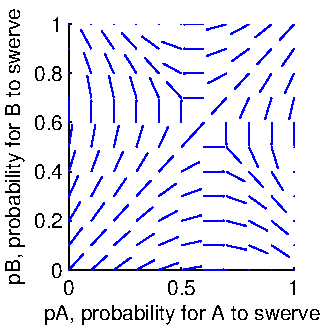
\includegraphics[scale=1.5]{ReplicatorDynamics2Dimensions.pdf}
\caption[]{Replicator Dynamics in 2 dimensions. The arrows indicate the direction of probability change}
\label{Rep2}
\end{figure}


In the well known Replicator Dynamics model in 2 Dimensions the Chicken Dilemma's behavior can be analysed demonstatively. In the Figure stated below it is obvious that for a certain starting vector $\left( \begin{array}{c} p_A \\ p_B \\ \end{array} \right) $ in the probabillity space a certain change of the probabillity vector will occur. Basically it can bee seen that if both players start at "high cooperation" they will both go in direction "low cooperation" and vice versa if both players start at "low cooperation". 
The starting vector is determining at which of the two equilibria states the probabillity vector finally will stay. Because of the symmetry in the usuall Chicken Dilemma it follows constructively that the line where $p_A$ = $p_B$ is the borderline for the two final equilibria. Hence, a slighly difference between the probability $p_A$ and $p_B$ determines the final equilibria state. This can be seen as well in the Figure. 
However, in stationary analysis, a third, non stationary equilibrium state can be calculated. Also this state is visible in Figure \ref{Rep2} at the probabillity vector of about v $\approx$ $\left( \begin{array}{c} 0.6 \\  0.6 \\ \end{array} \right) $. 
\newline

This unstable equilibrium state is also analytically calculated. Corresponding to \ref{edot} a equilibrium can be found by solving $\frac{d e_A}{d p_A}$ = 0 for $p_B$. This leads to
\begin{equation}
p_B = \frac{M_A(n,n) - M_A(c,n)}{M_A(c,c) - M_A(n,c) - M_A(c,n) + M_A(n,n)}
\end{equation} 
and vice versa solving for $\frac{d e_B}{d p_B}$ = 0 for $p_A$ leads to
\begin{equation}
p_A = \frac{M_B(n,n) - M_B(n,c)}{M_B(c,c) - M_B(c,n) - M_B(n,c) + M_B(n,n)}
\end{equation}

Inserting the values of tabular \ref{table11} will result exactly at a value of 0.6 for $p_A$ as for $p_B$ at the unstable equilibrium.



\begin{figure}[h]
\centering
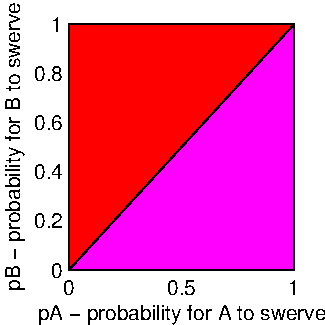
\includegraphics[scale=1.5]{PhaseDiagramm2D.pdf}
\caption{Symmetrical Chicken Dilemma. Areas indiacte final equilibirum state. Magenta: final state at $p_A$ = 1 and $p_B$ = 0, Red: final state at $p_A$ = 0 and $p_B$ = 1 }
\label{Phase1}
\end{figure}

The dynamics of an asymmetrical Chicken Dilemma are quiet different to those of a symmetrical one. In Figure \ref{Phase2} a Chicken Dilemma tabular of the following form has been implemented:

\begin{table}[htbp]
\centering
\begin{tabular}{|l|c|c|l|c|c|}

\hline
$ A | B $     &     Swerve  &    Straight    \\                           
\hline
$ Swerve $      &  1,  1     &  1,  3  \\
\hline
$ Straight $      &  3,  1    &  -2,  -10      \\
\hline
\end{tabular}

\label{table1} 
\caption{asymmetrical Chicken Dilemma with two players}

\end{table}

It can be seen that in case of A and B are both not cooperating, B will loose more than A does. This leads to more cooperation of player B - but not of player A. As expected, the diagramm of equilibira will change asymmetrically. Nevertheless, although there is a significant change of dynamics, the border between the final Nash Equilibria does stay a linear function. This can be explained analytically. The solutions of the trajectories corresponding to equation \ref{dgl} are still a linear combination of exponential functions because the parameters of the Matrix M are still constant - even though not symetrical. Thus there is a solution at which 
\begin{equation}
p_B(t) = C_o + C_s \cdot p_A(t)
\end{equation}
where $C_o$ is  the offset constant and $C_s$ the slope of the line.
\newline 


\begin{figure}[h]
\centering
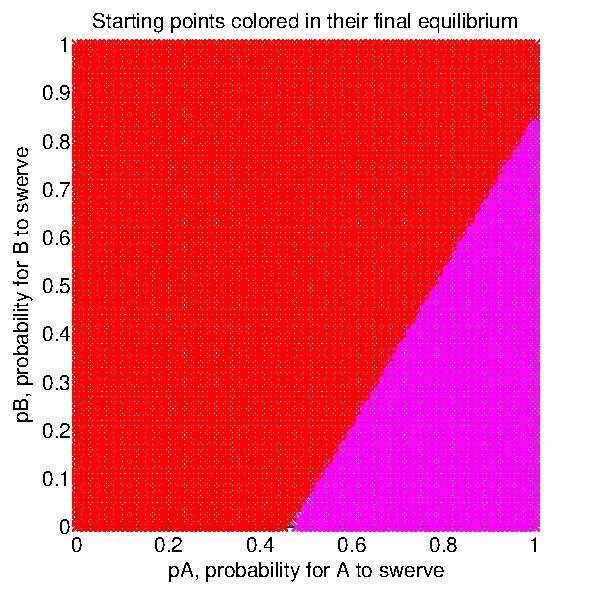
\includegraphics[scale=1]{PhaseDiagramm2Da.pdf}
\caption{Asymmetrical Chicken Dilemma. Colors indiacte final equilibirum state at each starting point. Magenta: final state at $p_A$ = 1 and $p_B$ = 0, Red: final state at $p_A$ = 0 and $p_B$ = 1 }
\label{Phase2}
\end{figure}

For the analysis of a corruption dependent punishment it has been assumed that the punishment is proportional to the cooperation. So that 
\begin{equation}
M(n,n) = (p_A + p_B) \cdot (-2)
\end{equation}
Thus the tabular looks like the following one:
\begin{table}[htbp]
\centering
\begin{tabular}{|l|c|c|l|c|c|}

\hline
$ A | B $     &     Swerve  &    Straight    \\                           
\hline
$ Swerve $      &  1,  1     &  1,  3  \\
\hline
$ Straight $      &  3,  1    &  ($p_A$ + $p_B$) $\cdot$ (-2),  ($p_A$ + $p_B$) $\cdot$ (-2)      \\
\hline
\end{tabular}

\label{probdependent} 
\caption{probability dependent Chicken Dilemma with two players}

\end{table}

What can be cleary seen in Figure \ref{Phase2Db} is that a third Nash Equilibrium occurs in case of a probability dependent punishment. This result fits well to intuition: In case of both players do rarely cooperate, the punishment will be low so that no need for a cooperator is required. Both players tend to corruption even more and will finally end up in total corruption!
The Chicken Dilemma referred to tabular \ref{probdependent} has been expressed in form of a differential equation for getting a look inside more closely.
\begin{equation}
\begin{split}
\frac{d p_A}{dt} = - 2 \cdot p_B - (p_B - 1) \cdot (4 \cdot p_A + 2 \cdot p_B - 1) \\ \frac{d p_B}{dt} = - 2 \cdot p_A - (p_A - 1) \cdot (4 \cdot p_B + 2 \cdot p_A - 1)
\end{split}
\end{equation}
As can be seen, this system is nonlinear. The solutions will not be anymore superimposed exponential functions. 


\begin{figure}[h]
\centering
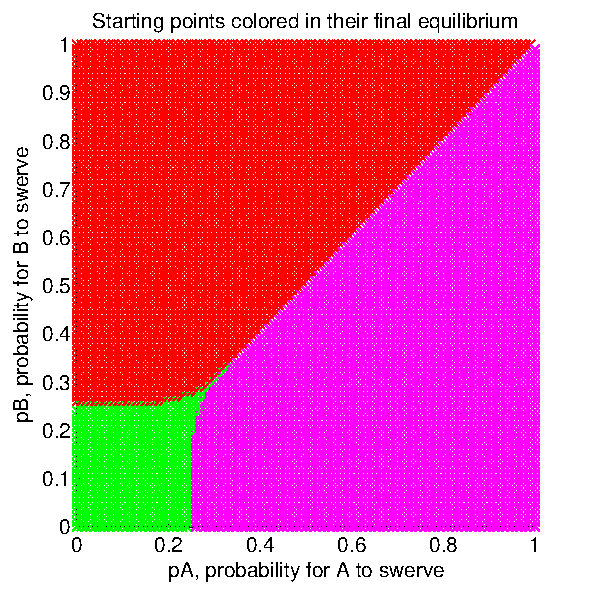
\includegraphics[scale=1]{PhaseDiagramm2Db.pdf}
\caption{Probability dependent Chicken Dilemma. Colors indicate final equilibrium state at each starting point. Magenta: final state at $p_A$ = 1 and $p_B$ = 0, Red: final state at $p_A$ = 0 and $p_B$ = 1, Green: final state at $p_A$ = $p_B$ = 0}
\label{Phase2Db}
\end{figure}

\newpage

\begin{figure}[h]
\centering
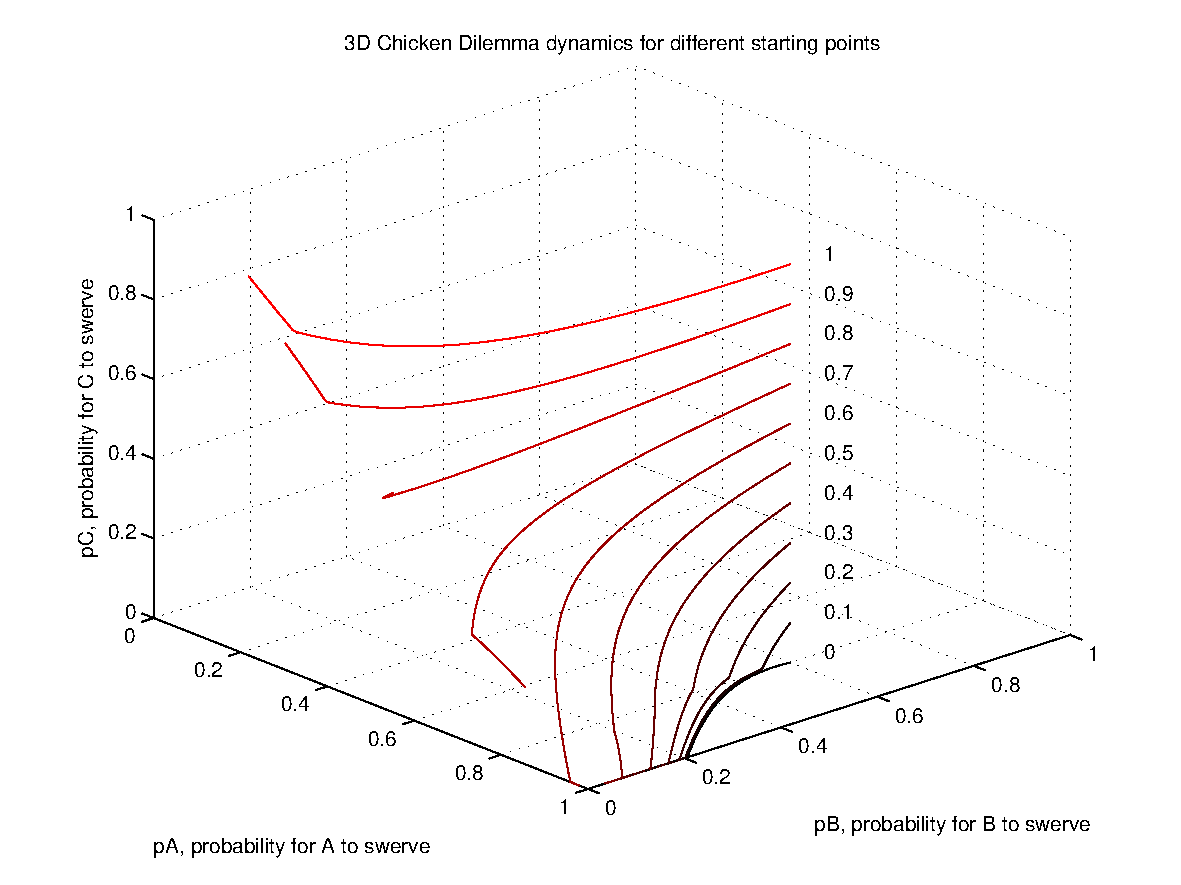
\includegraphics[scale=0.7]{ReplicatorDynamics3Dimensions2.pdf}
\caption[Replicator Dynamics in 3 Dimensions]{Trajectories of Replicator Dynamics in 3 dimensions for different starting points. 
Starting points are at locations $p_A$ = 0.8, $p_B$ = 0.6 and $p_C$ is iterated from 0 to 1 in a step size of 0.1}
\label{Rep31}
\end{figure}

For the Replicator Dynamics of the Chicken Dilemma in 3 dimensions the trajectories in Figure show the path of evolution in probability space. In 3 dimensions it is possible to reach a certain state in more different ways than you could do in 2 dimensions. This is exactly what is behind the Chicken Dilemma extended to 3 dimensions. The difference is, that the probability state of a third player $p_C$ influences the behavior of player A and B. Assuming player A and player B would play only against each other, they would take a different decision than they would take in case of player C is joining. Thus an additional player C leads to a more complex behavior of player A and B. Assuming a realistic model where the probabilites of player A and B are known but not the one of player C, this may explain why it is not possible to forecast the outcome in certain - even  more complex - situations. 
In 3 dimensions there are three stable equilibria. These follow from all combinations of two players do not cooperate and one cooperates. The equilibria at which two players do cooperate and one does not are not stable. This can be seen easily by looking at \ref{table2}. Assuming player A and B do cooperate but player C does not. The values in the table for A and B look now equivalent compared to the ones in the 2-dimensional Chicken Dilemma where we do not have a stable equilibrium for A and B cooperating.
\newline


\begin{figure}[h]
\centering
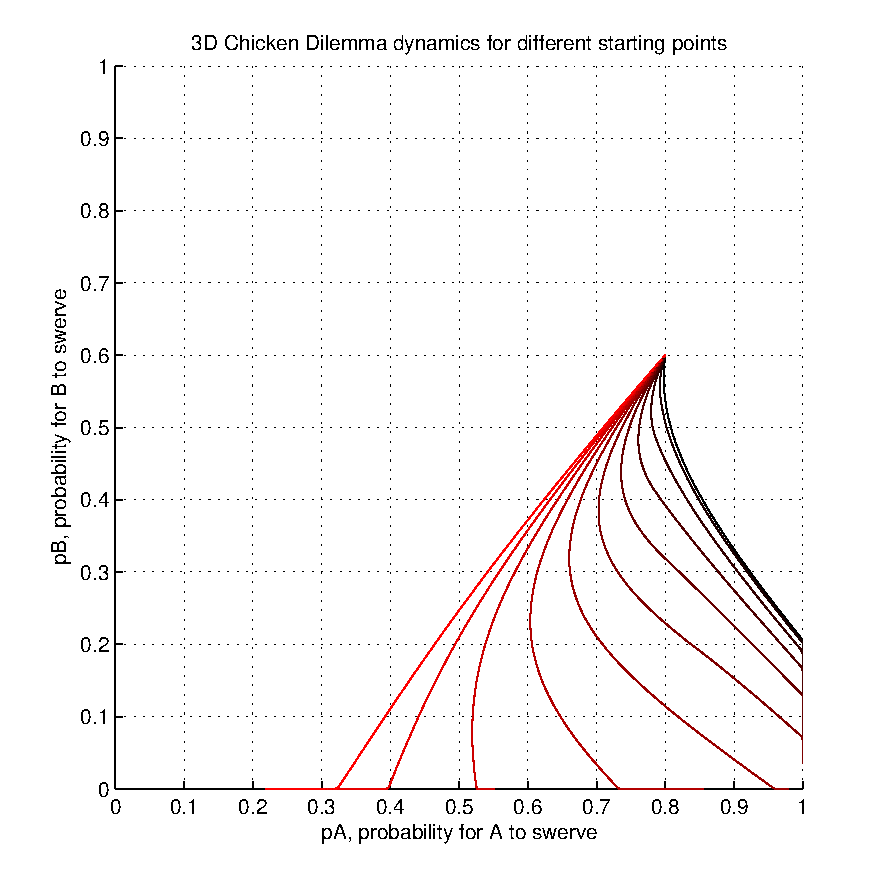
\includegraphics[scale=0.69]{ReplicatorDynamics3Dimensions1.pdf}


\caption[Replicator Dynamics in 3 Dimensions]{Projection on the $p_A$ - $p_B$ - axis of Replicator Dynamics in 3 dimensions. Every color represents the trajectory of a different starting point where $p_C$ is iterated from 0 to 1 in a step size of 0.1}
\label{Rep32}

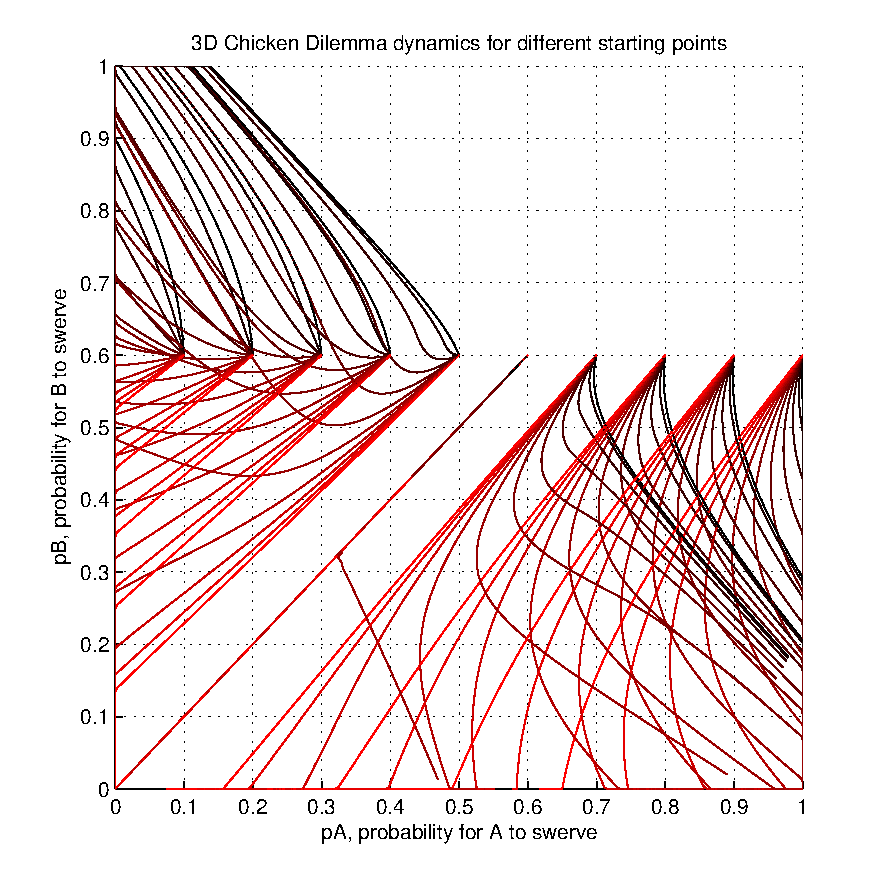
\includegraphics[scale=0.69]{ReplicatorDynamics3Dimensions3.pdf}
\caption[Replicator Dynamics in 3 Dimensions]{Projection on the $p_A$ - $p_B$ - axis of Replicator Dynamics in 3 Dimensions. Every color represents a different starting probability $p_C$. $p_A$ and $p_C$ are iterated from 0 to 1 in a step size of 0.1. }
\label{Rep33}

\end{figure}


In Figure 4 different evolution trajectories are shown. As mentioned above it is obvious that for different starting probabilities $p_C$ different trajectories occur. Moreover, as can be seen that the trajectories may go into totally different directions and finally different equilibria states. A certain threshold probability $p_C$ $\approx$ 0.8 is identifiable for which different equilibria are reached. This can be well seen in Figure \ref{Rep32}. 
In addition, it is important to mention that the trajectories in the perspective of Figure \ref{Rep32} do not ressemble those in the 2-dimensional Replicator Dynamics. This is because  a certain value $p_C$ leads to a different direction change in probability between $p_A$ and $p_B$.
\newline

In Figure \ref{Rep33} only the probability $p_B$ has not been varied. As can be seen lines "cross" each other in this perspective. This shows again how the trajectory depends on the probability $p_C$. Moreover, for $p_A$ = $p_B$ every change in $p_A$ will be equal to the change in $p_B$.




\begin{figure}[h]
\centering
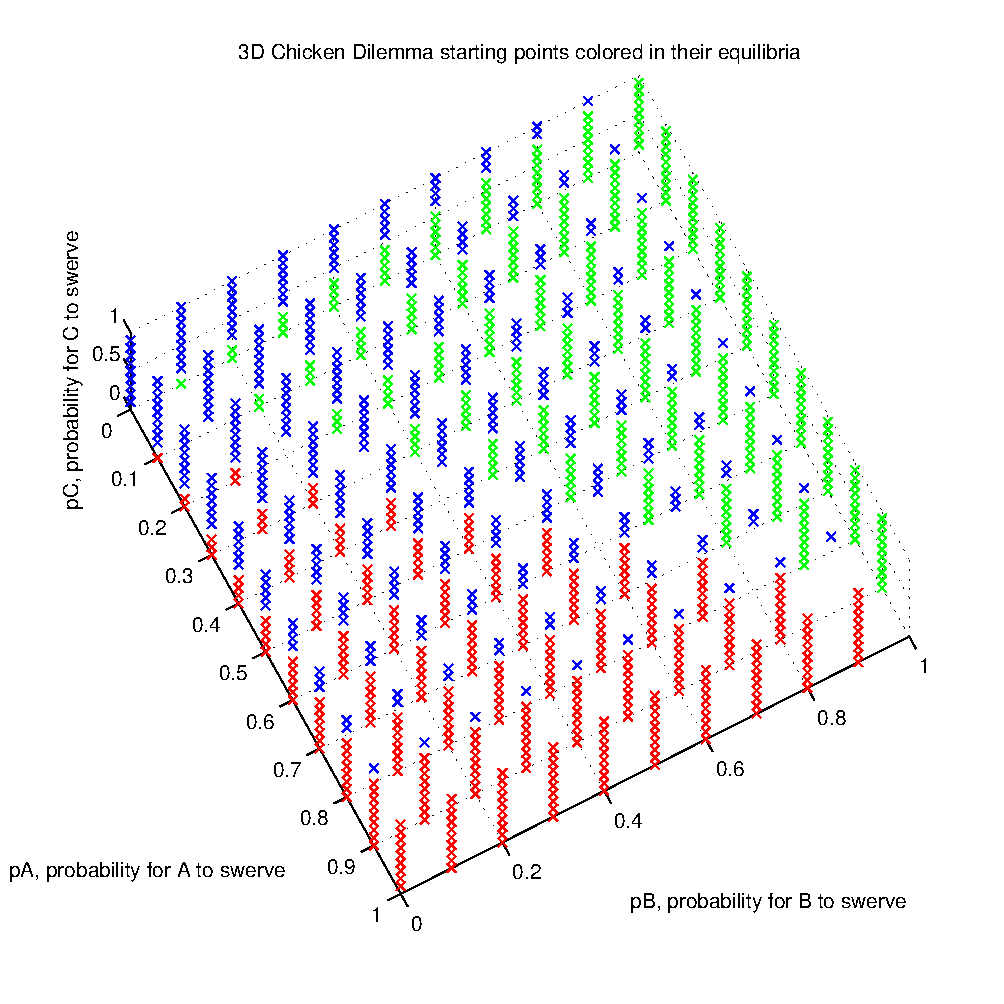
\includegraphics[scale=1]{PhaseDiagramm3D.pdf}
\caption[]{Colors indiacte final equilibirum state at each starting point. The equilibirum states for each color are: 
 Red: $p_A$ = 1, $p_B$ = 0 and $p_C$ = 0, Green: $p_A$ = 0, $p_B$ = 1 and $p_C$ = 0, Blue: $p_A$ = 0, $p_B$ = 0 and $p_C$ = 1. Notice that there are some non-colored starting points because the simulation result would have taken too long}
\label{Phase3}
\end{figure}


\subsection{3x3 Cellular Automaton}

The evolution of probabilities with increasing steps is shown in Figure \ref{cell1}. What can be clearly seen on the simple but instructive model at the 3x3 player Cellular Automaton is that it will alyways end up at one player will do the opposite to all other players. In this simple implementation although the weight of the Chicken Dilemma table has been fully neglected it will lead to a stable equilibrium. But it has to been mentioned that it is not clearly guaranteed at which state the player ends up. One equilibrium is that 8 players end up and probability 1 and player number 9 at probability 0 and vice versa. 
This model does not say anything about the Chicken Dilemma itself but it does show the outcome of players doing corruption if others do not and vice versa neglecting expection values.

\begin{figure}[h]
\centering
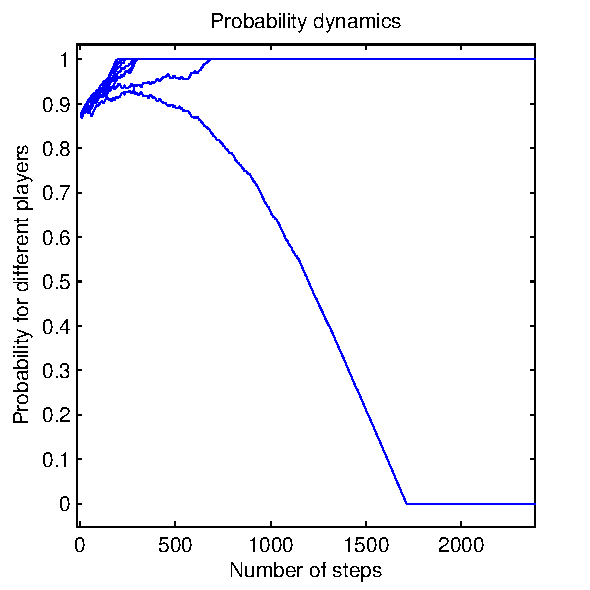
\includegraphics[scale=1]{ProbabilityDynamics1.pdf}
\caption{Probability dynamics of 9 players playing against each other - one player will go into other strategy than the rest of the players}
\label{cell1}
\end{figure}













\subsection{Cellular Automaton}

%%%%%%%%%%%%%%%%%%%%%%%%%%%%%%%%%%%%%%%%%%%%%%%%%%%%%%%%%%%%%%%%%%%%%%%%%%%

%%%%%%%%%%%%%%%%%%%%%%%%%%%%%%%%%%%%%%%%%%%%%%%%%%%%%%%%%%%%%%%%%%%%%%%%%%%
With our Implementation of the Chicken Dilemma, we tested several scenarios. It is remarkably, that if one defines uniform initial conditions for all player, no matter what strategy one defines, there won't build any cluster of equal probabilities of cooperation. As an example we state the case where one has uniform initial aspirations of 3, and all players decide first randomly. The strategy is chosen as Learning as described in our model without peer pressure. In figure \ref{exp1time} one can see that the probabilitie of cooperation moves always around 0.5 and has no tendence to fall or climb.

\begin{figure}
\centering
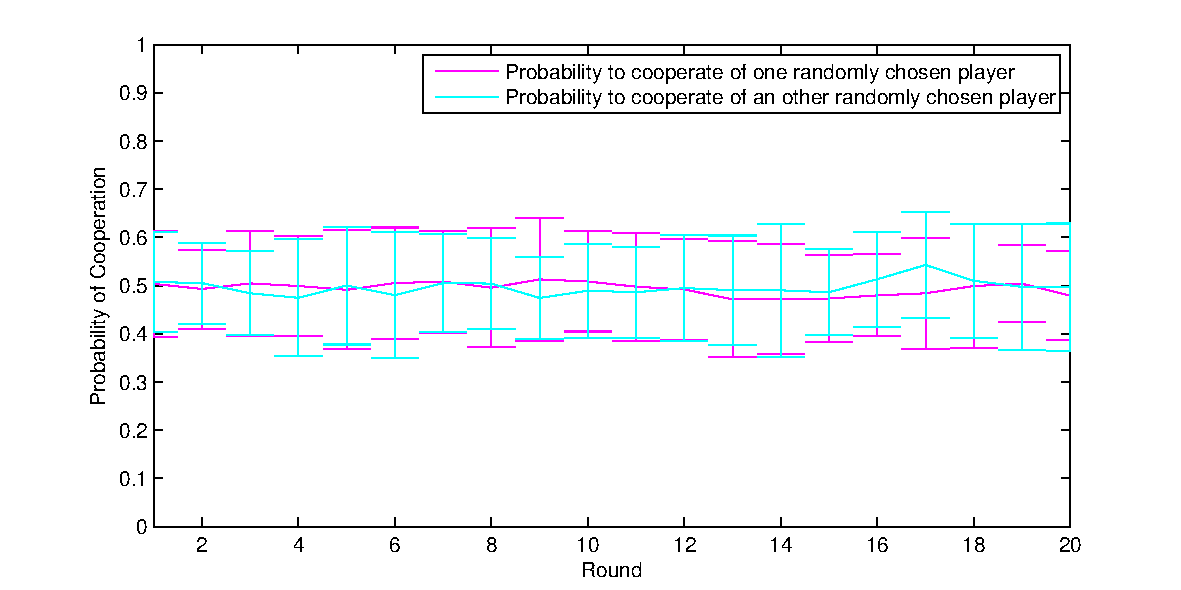
\includegraphics[scale=0.8]{ProbCoopwithtime1.pdf}
\caption[]{This is the probability for cooperation for 2 Players plottet for each round. One played over 20 rounds with 400 players and middled over 40 simulations. The initial conditions were set such that: the aspiration is 3 for all players, the probability for cooperation is 0.5 for everybody and each player has the strategy of learning with a learning rate of 0.8. }
\label{exp1time}
\end{figure}

In an other experiment we examined what happens if one chooses a uniform initial aspiration of 3, the strategy of learning with peer pressure for all players and on one hand an initial distribution of probability to cooperate of the form as sinusoidal \ref{exp19} or floating from the top to the bottom \ref{exp20}.

\begin{figure}
\centering
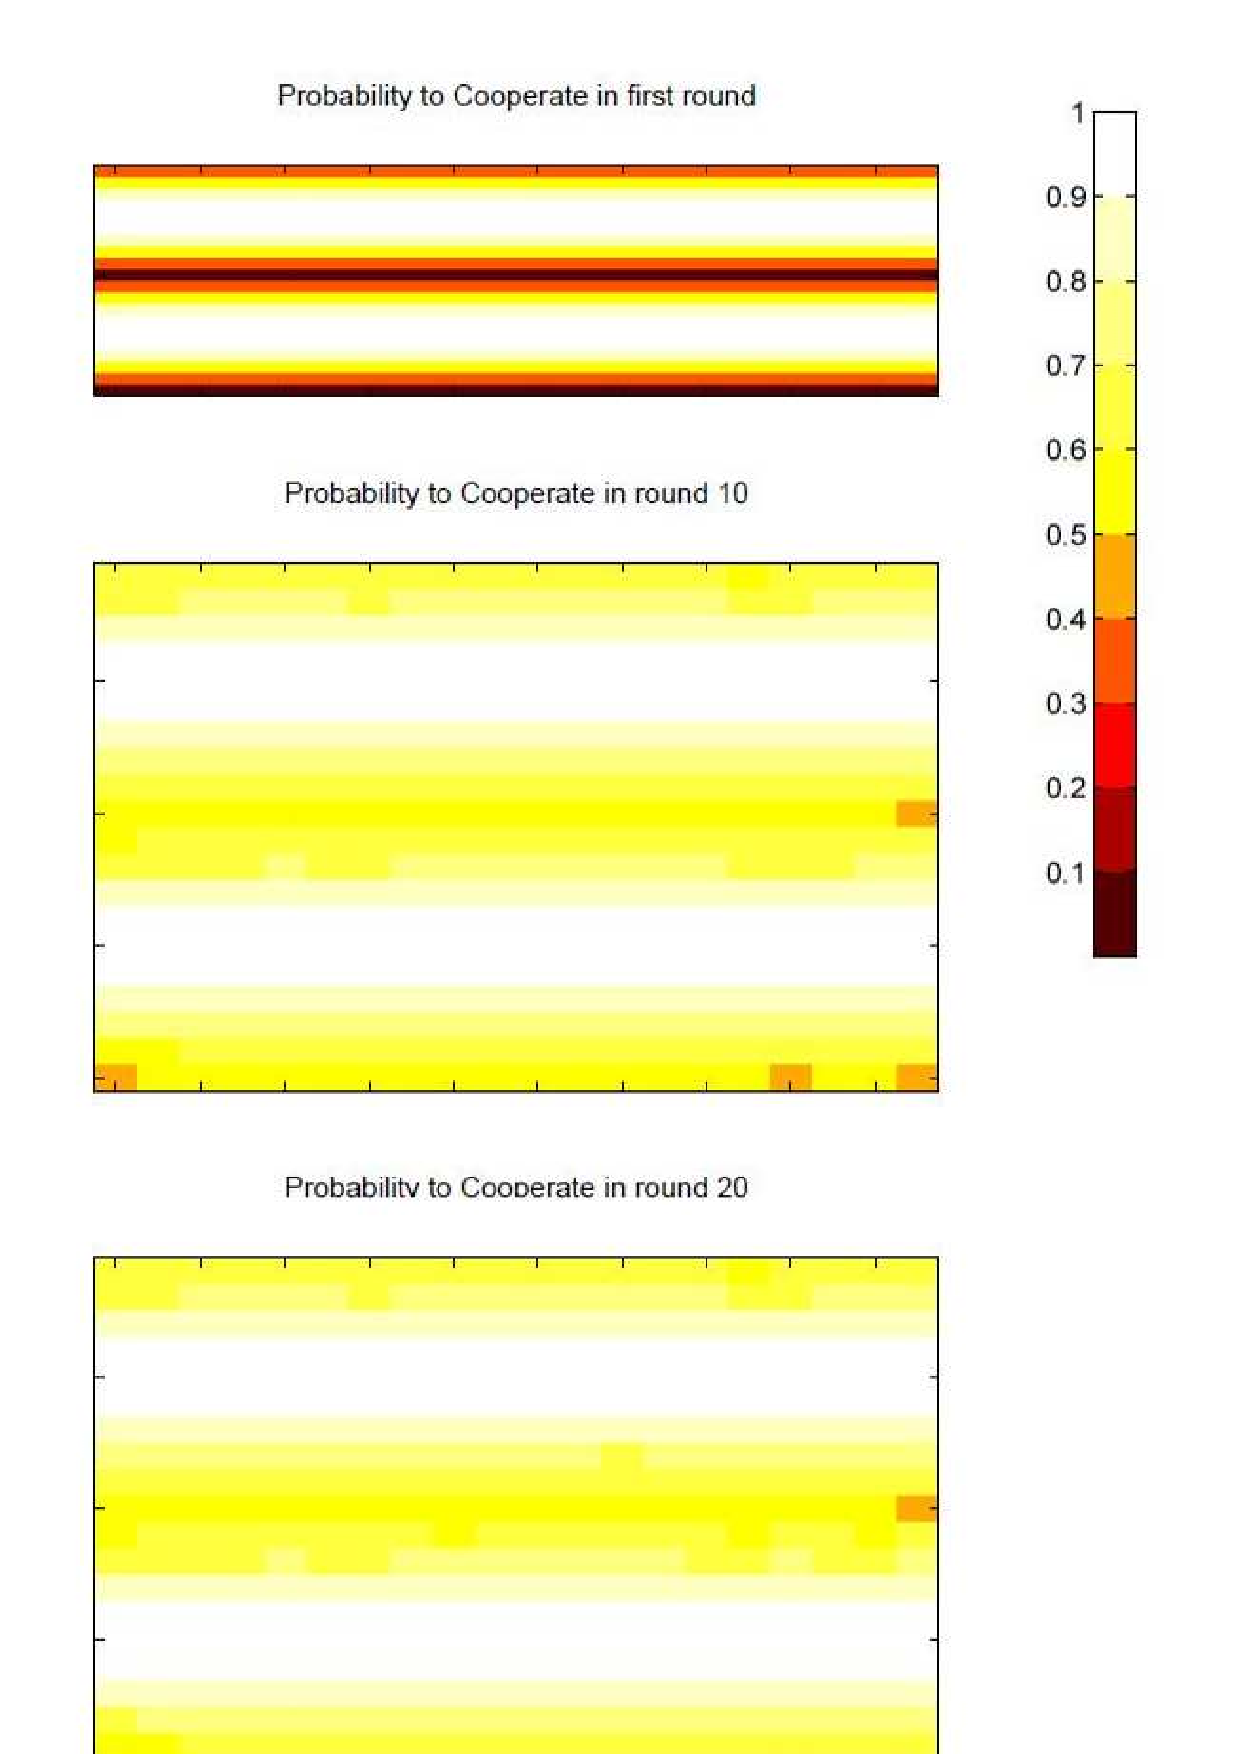
\includegraphics[scale=0.4]{ProbabilityToCooperateInDiffRound19.pdf}
\caption[]{This is the probability for cooperation each Player for 3 rounds ( 1 , 10 and 20). One played over 50 rounds with 400 players and middled over 40 simulations. The initial conditions were set such that: the aspiration is 3 for all players, the probability for cooperation is sinusoidal distributed from 1 to 0 and everybody has the strategy of learning with peer pressure  with a learning rate of 0.8. }
\label{exp19}
\end{figure}

\begin{figure}
\centering
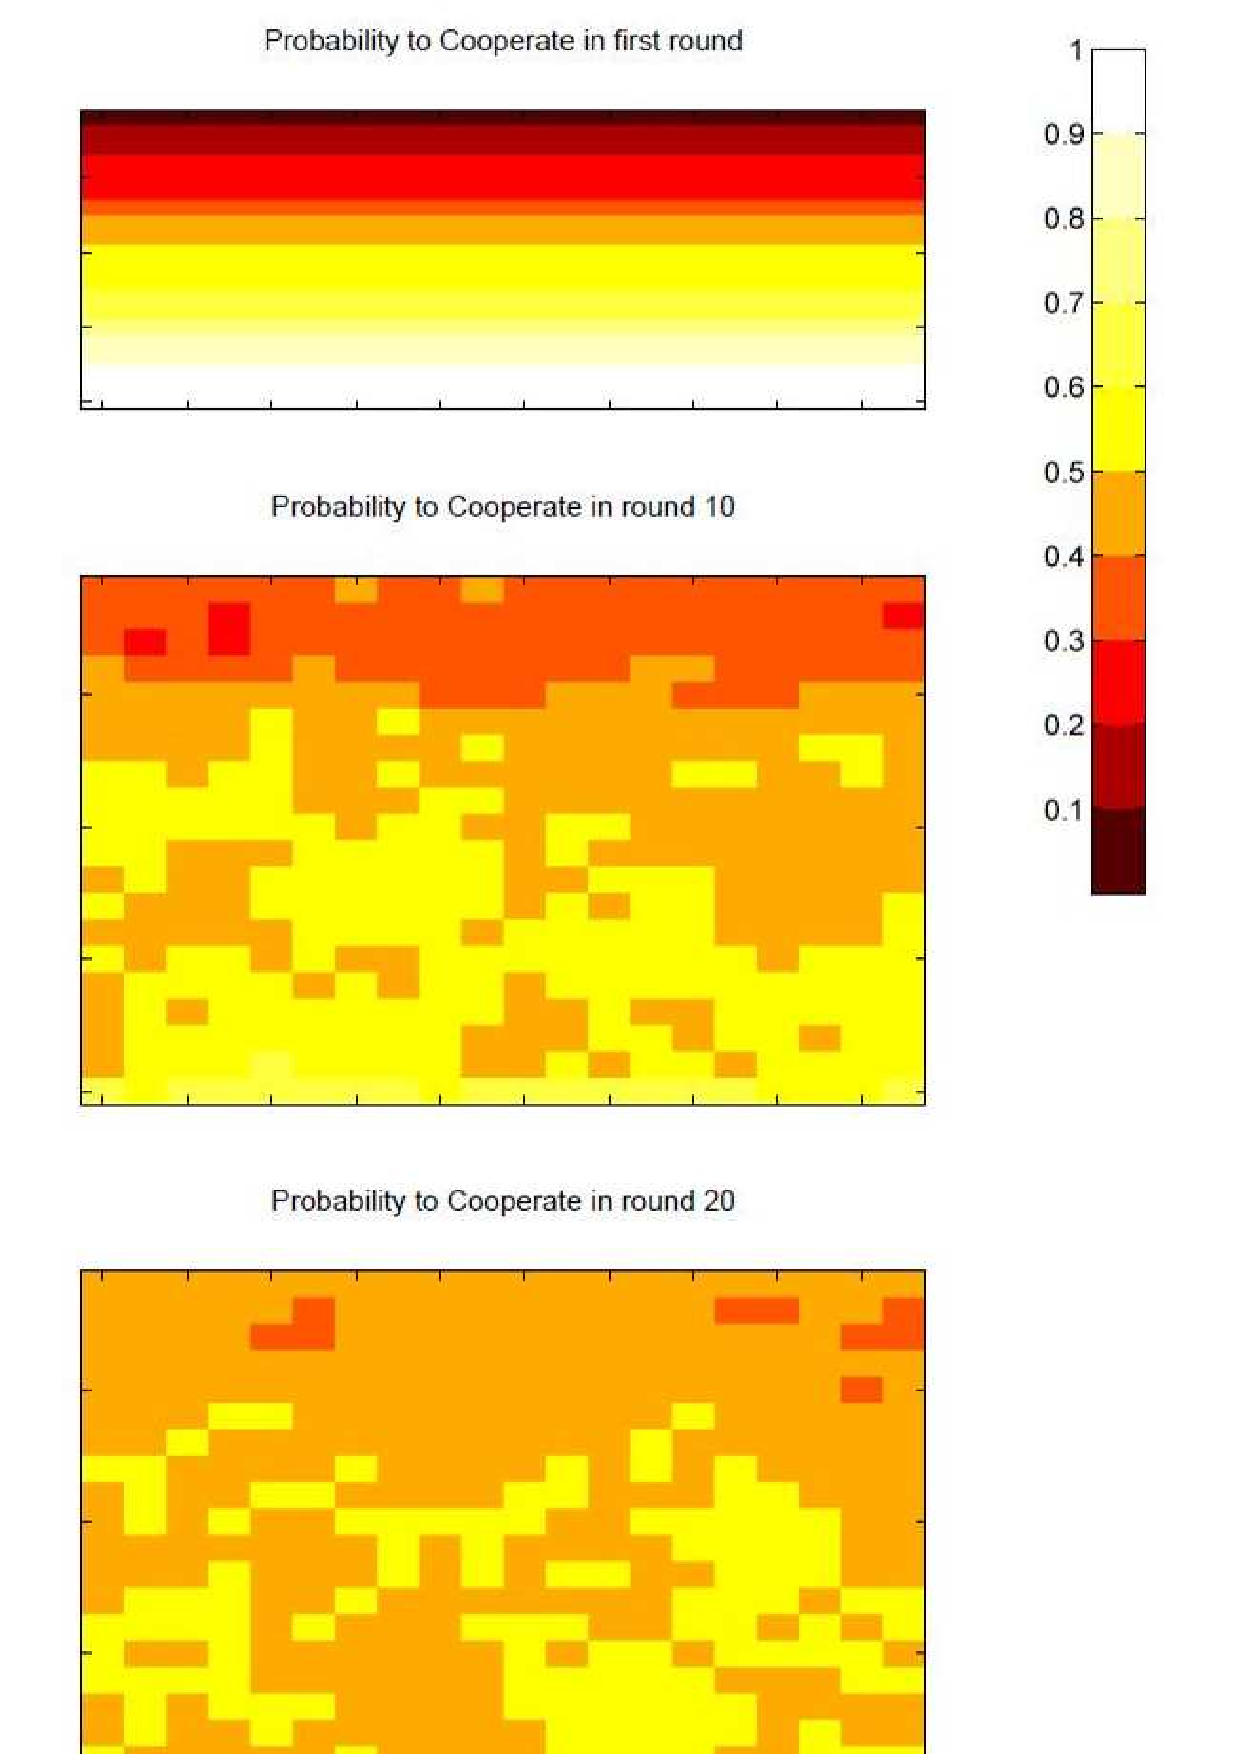
\includegraphics[scale=0.4]{ProbabilityToCooperateInDiffRound20.pdf}
\caption[]{This is the probability for cooperation each Player for 3 rounds ( 1 , 10 and 20). One played over 50 rounds with 400 players and middled over 40 simulations. The initial conditions were set such that: the aspiration is 3 for all players, the probability for cooperation is floatingl distributed from 1 to 0 and everybody has the strategy of learning with peer pressure  with a learning rate of 0.8. }
\label{exp20}
\end{figure}

One can see that in the case of a sinusoidal probability distribution it smooves out a little bit with higher rounds, but then keeps its shape. This can also bee seen in figure \ref{exp20time}. But the floating one smooves out completely.


\begin{figure}
\centering
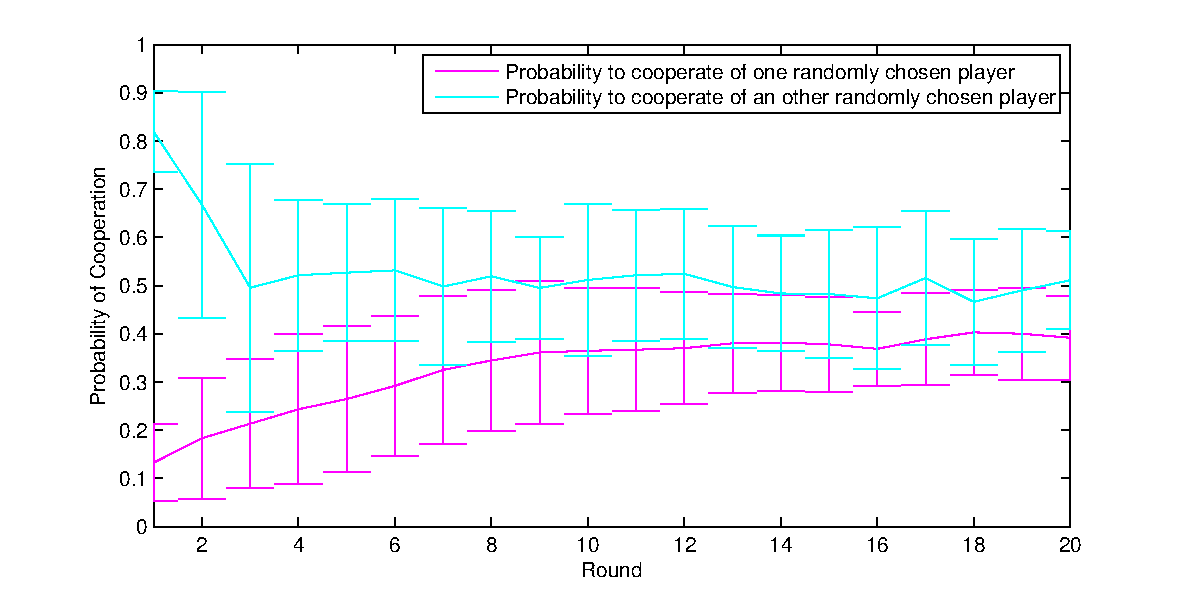
\includegraphics[scale=0.8]{ProbCoopwithtime20.pdf}
\caption[]{This is the probability for cooperation for 2 Players (one from the top and one from the bottom) plottet for each round. The initial conditions were set such that: the aspiration is 3 for all players, the probability for cooperation is floatingl distributed from 1 to 0 and everybody has the strategy of learning with peer pressure  with a learning rate of 0.8.}
\label{exp20time}
\end{figure}


In figure \ref{exp14} one can see the effect of varying initial aspirations. We defined an initial aspiration of 2 for the players in the half at the top, and 4 for the rest.
\\The initial probability of cooperation was uniformly chosen as 0.5 and the strategy was defined as learning with peer pressure, where the decisions of the neigbourhood of the 3 last games was taken into account.

\begin{figure}
\centering
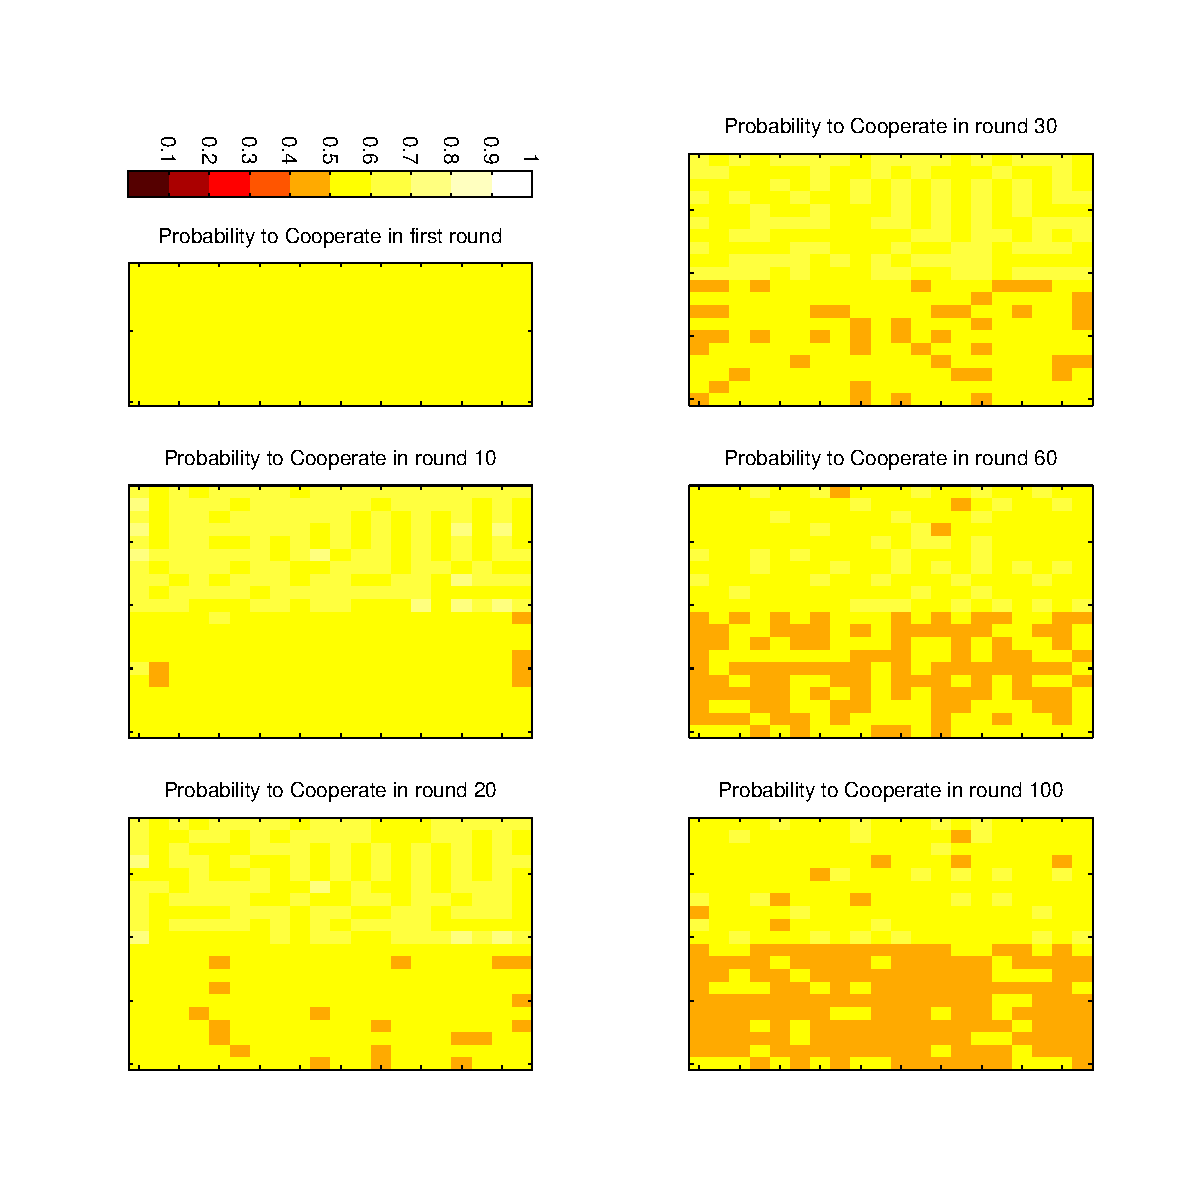
\includegraphics[scale=0.6]{ProbabilityToCooperateInDiffRound14.pdf}
\caption[]{This is the probability for cooperation each Player for 6 rounds ( 1 , 10, 20, 30, 60 and 100). One played over 50 rounds with 400 players and middled over 40 simulations. The initial conditions were set such that: the aspiration is 2 for players in the upper half of the field and 4 for the rest, the initial probability for cooperation is 0.5 for everyone and everybody has the strategy of learning with peer pressure taking 3 decisions of the neighbourhood in the past into account as described before with a learning rate of 0.8. }
\label{exp14}
\end{figure}

One can see that the ones with the initially higher aspiration starts to deflect a bit more, where as the others start between round 60 and 100 also slighty to defect.
\\When one starts with the initial conditions were set such that: the aspiration is 3 for all players, the probability for cooperation is 1 and everybody has the strategy of learning with a learning rate of 0.8 one can see that the probability to cooperate stabilizes at around 0.5.\ref{exp31}

\begin{figure}
\centering
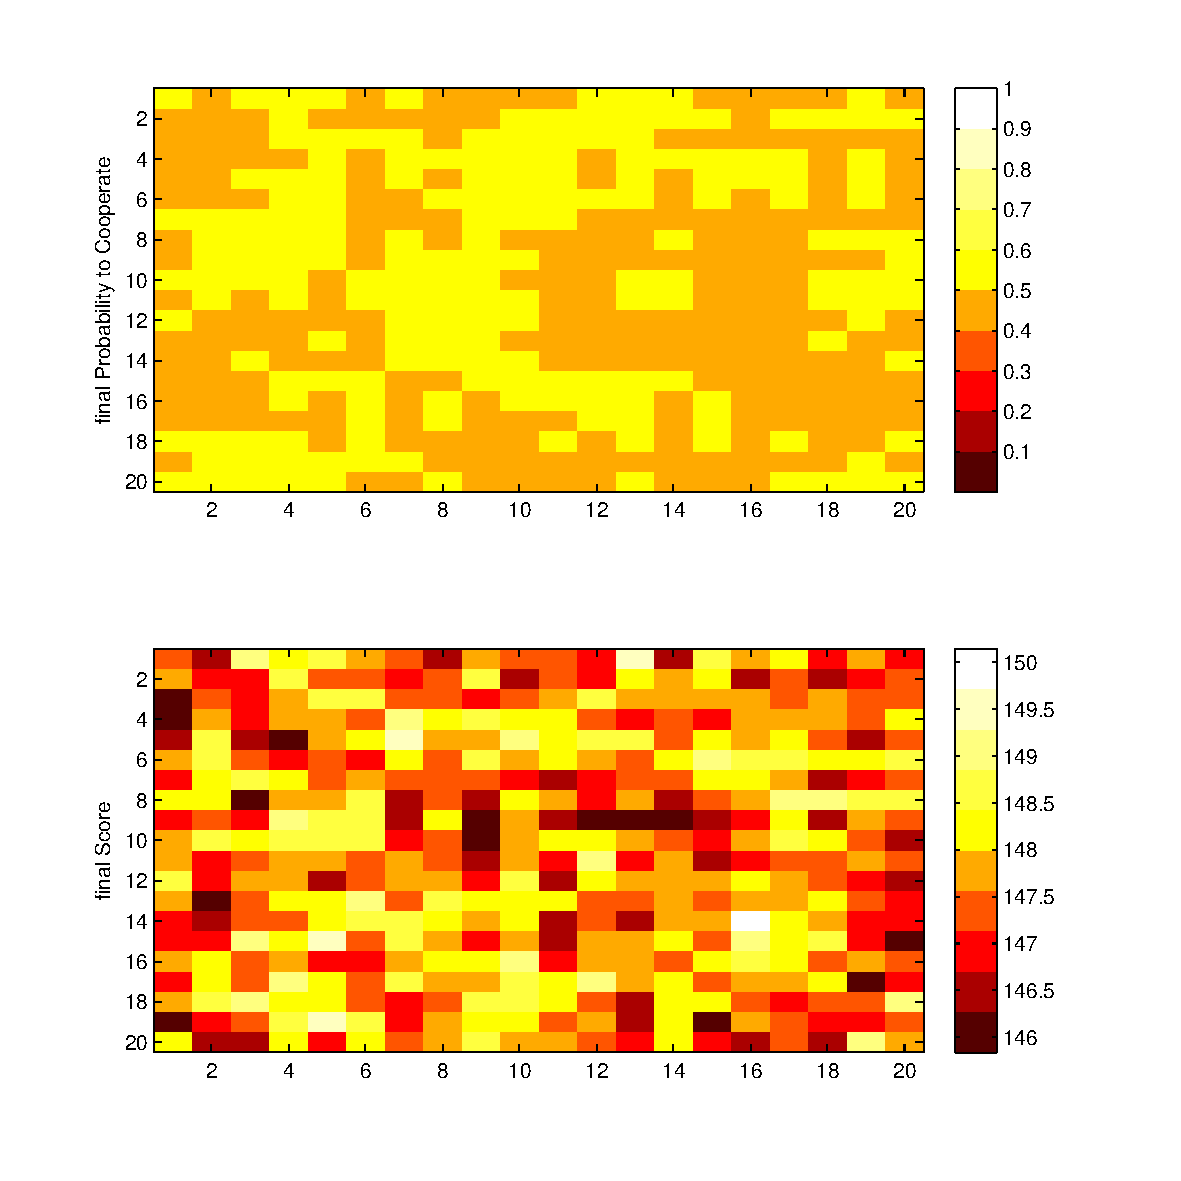
\includegraphics[scale=0.6]{ScoreAndProbcoopWithImagesc_0_1_31.pdf}
\caption[]{This is the final probability for cooperation and the score of each Player. One played over 50 rounds with 400 players and middled over 40 simulations. The initial conditions were set such that: the aspiration is 3 for all players, the probability for cooperation is 1 and everybody has the strategy of learning with a learning rate of 0.8.}
\label{exp31}
\end{figure}


In the next experiment, we examined how our built in peer pressure effects the result. In figure \ref{exp11} we took the strategy of leraning without and in figure \ref{exp12} with peer pressure. The initial conditions were set such that: the aspiration is 2 for players in the upper half of the field and 4 for the rest, the initial probability for cooperation is 0.5 for everyone and everybody has the strategy of learning without peer pressure with a learning rate of 0.8. If one compares the two figures, on remarks that there no big difference. Each systems learn as fast. We made other experiments where a neighbourhood has one time a lower initial probability of cooperation and the other time a higher. If one chooses the Strategy of the neighbourhood as Learning and the rest constantly decides with initial probability one get the following:
\\If neighbourhood $P(cooperation)=0.5$, others$P(cooperation)=0.7$ then it always tooks them in mean 48.8 rounds to converge themselfs up to 1% with or without peer pressure.
\\If neighbourhood $P(cooperation)=0.5$, others$P(cooperation)=0.2$ they don't converge but stay around $P(cooperation)=0.5$ as shown in figure \ref{exp35atime}.

\begin{figure}
\centering
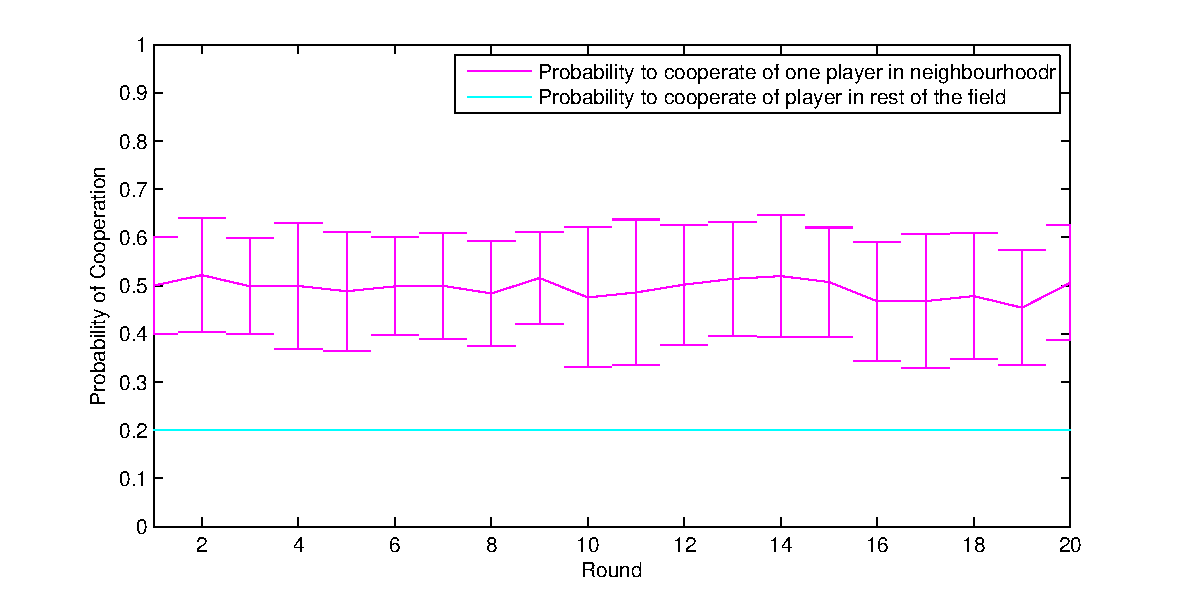
\includegraphics[scale=0.8]{ProbCoopwithtime35a.pdf}
\caption[]{This is the probability for cooperation for 2 Players plottet for each round. One played over 20 rounds with 400 players and middled over 40 simulations. The initial conditions were set such that: the aspiration is 3 for all players, the probability for cooperation is 0.5 for a chosen neighbourhood which has the strategy of learning with a learning rate of 0.8 and the rst has the initial probability to cooperate of only 0.2 and keep this conditions over the whole game.}
\label{exp35atime}
\end{figure}

\begin{figure}
\centering
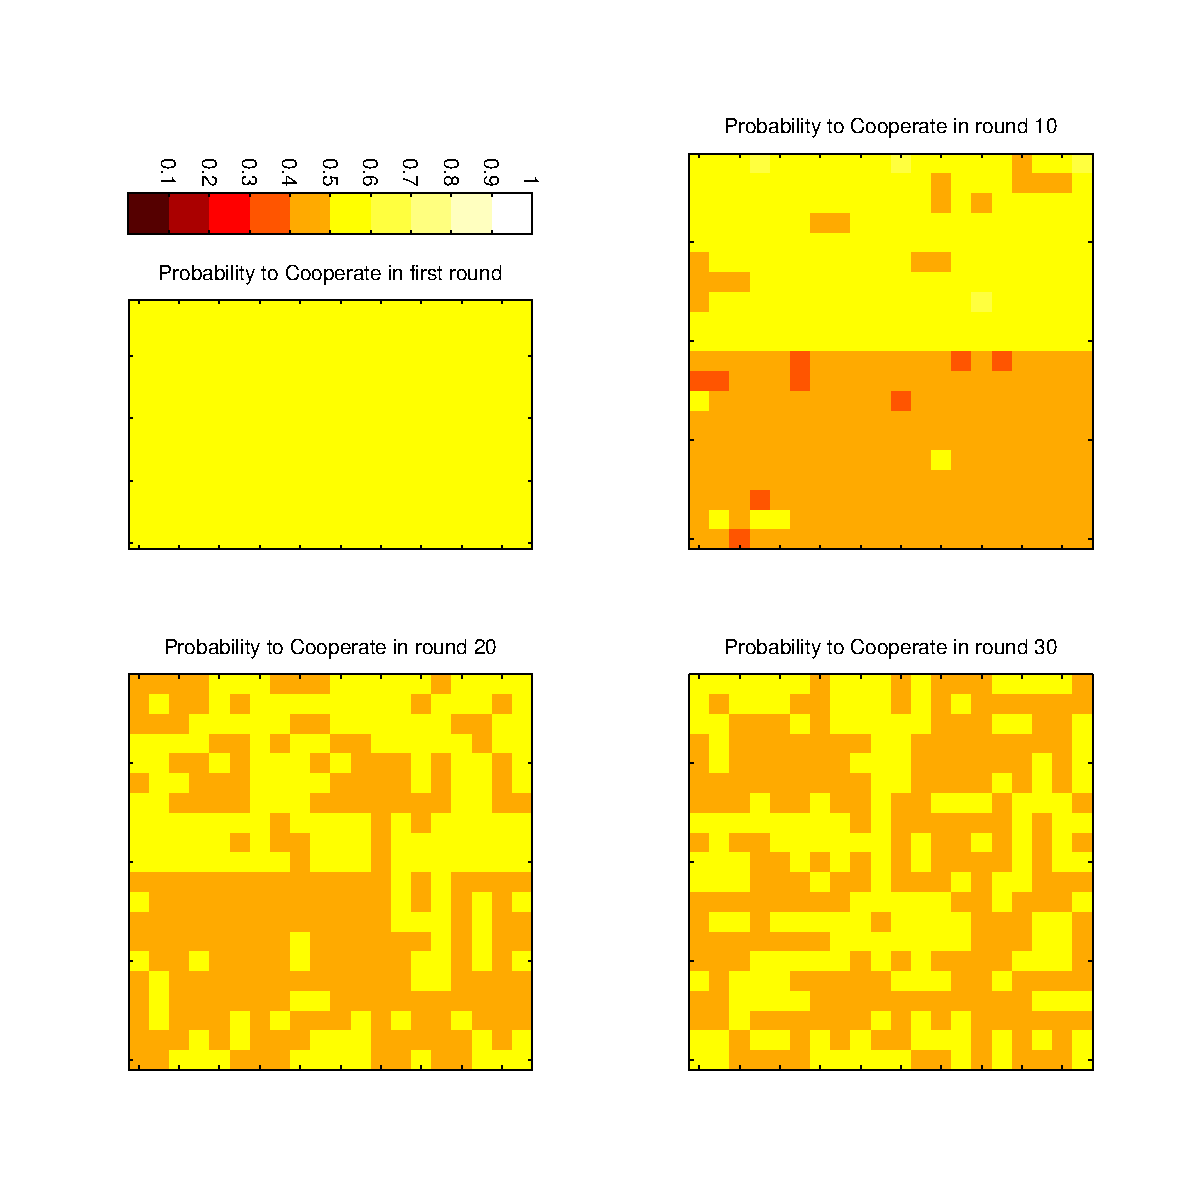
\includegraphics[scale=0.6]{ProbabilityToCooperateInDiffRound11.pdf}
\caption[]{This is the probability for cooperation each Player for 4 rounds ( 1 , 10, 20 and 30). One played over 50 rounds with 400 players and middled over 40 simulations. The initial conditions were set such that: the aspiration is 2 for players in the upper half of the field and 4 for the rest, the initial probability for cooperation is 0.5 for everyone and everybody has the strategy of learning without peer pressure with a learning rate of 0.8. }
\label{exp11}
\end{figure}

\begin{figure}
\centering
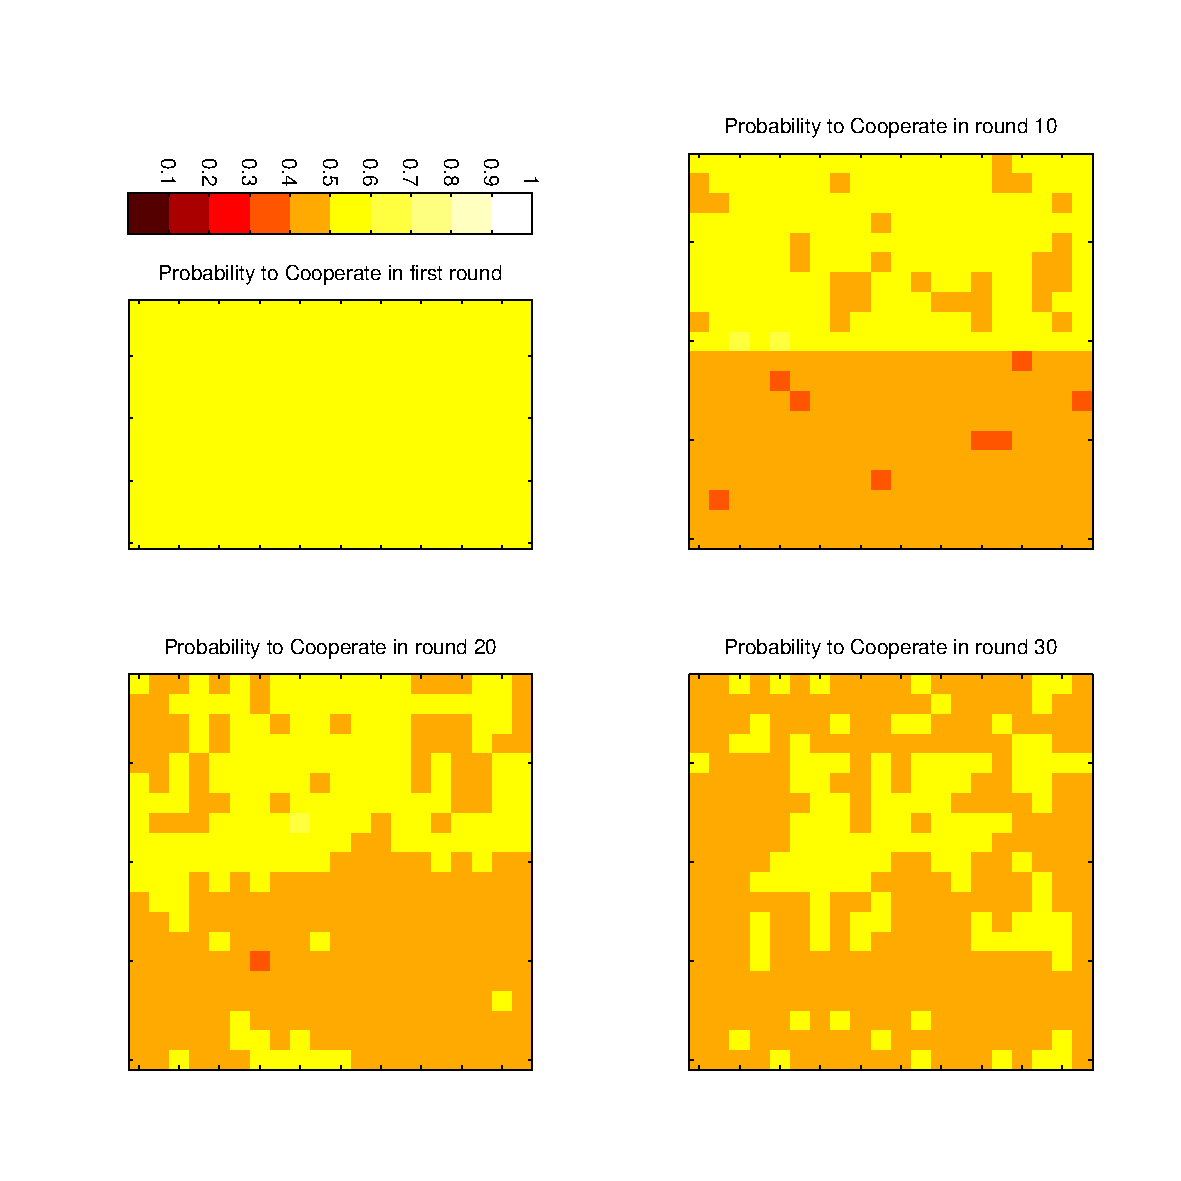
\includegraphics[scale=0.6]{ProbabilityToCooperateInDiffRound12.pdf}
\caption[]{This is the probability for cooperation each Player for 4 rounds ( 1 , 10, 20 and 30). One played over 50 rounds with 400 players and middled over 40 simulations. The initial conditions were set such that: the aspiration is 2 for players in the upper half of the field and 4 for the rest, the initial probability for cooperation is 0.5 for everyone and everybody has the strategy of learning with peer pressure with a learning rate of 0.8. }
\label{exp12}
\end{figure}
In the next experiment we examined how much the learning rate effects the system.  The initial conditions were set such that: the aspiration is for everybody 3, the initial probability for cooperation is1 for everyone. The strategy is distributed such that the upper half of the players have a lower learning rate (0.5) then the rest (0.8). This is described with figure \ref{exp30} and \ref{exp30time}. It is nicely shown, that first the ones with higher learning rate immediately start to deflect before the ones with the lower learning rate follow and then it stabilizes where everybody has $P(cooperation)=0.5$. 

\begin{figure}
\centering
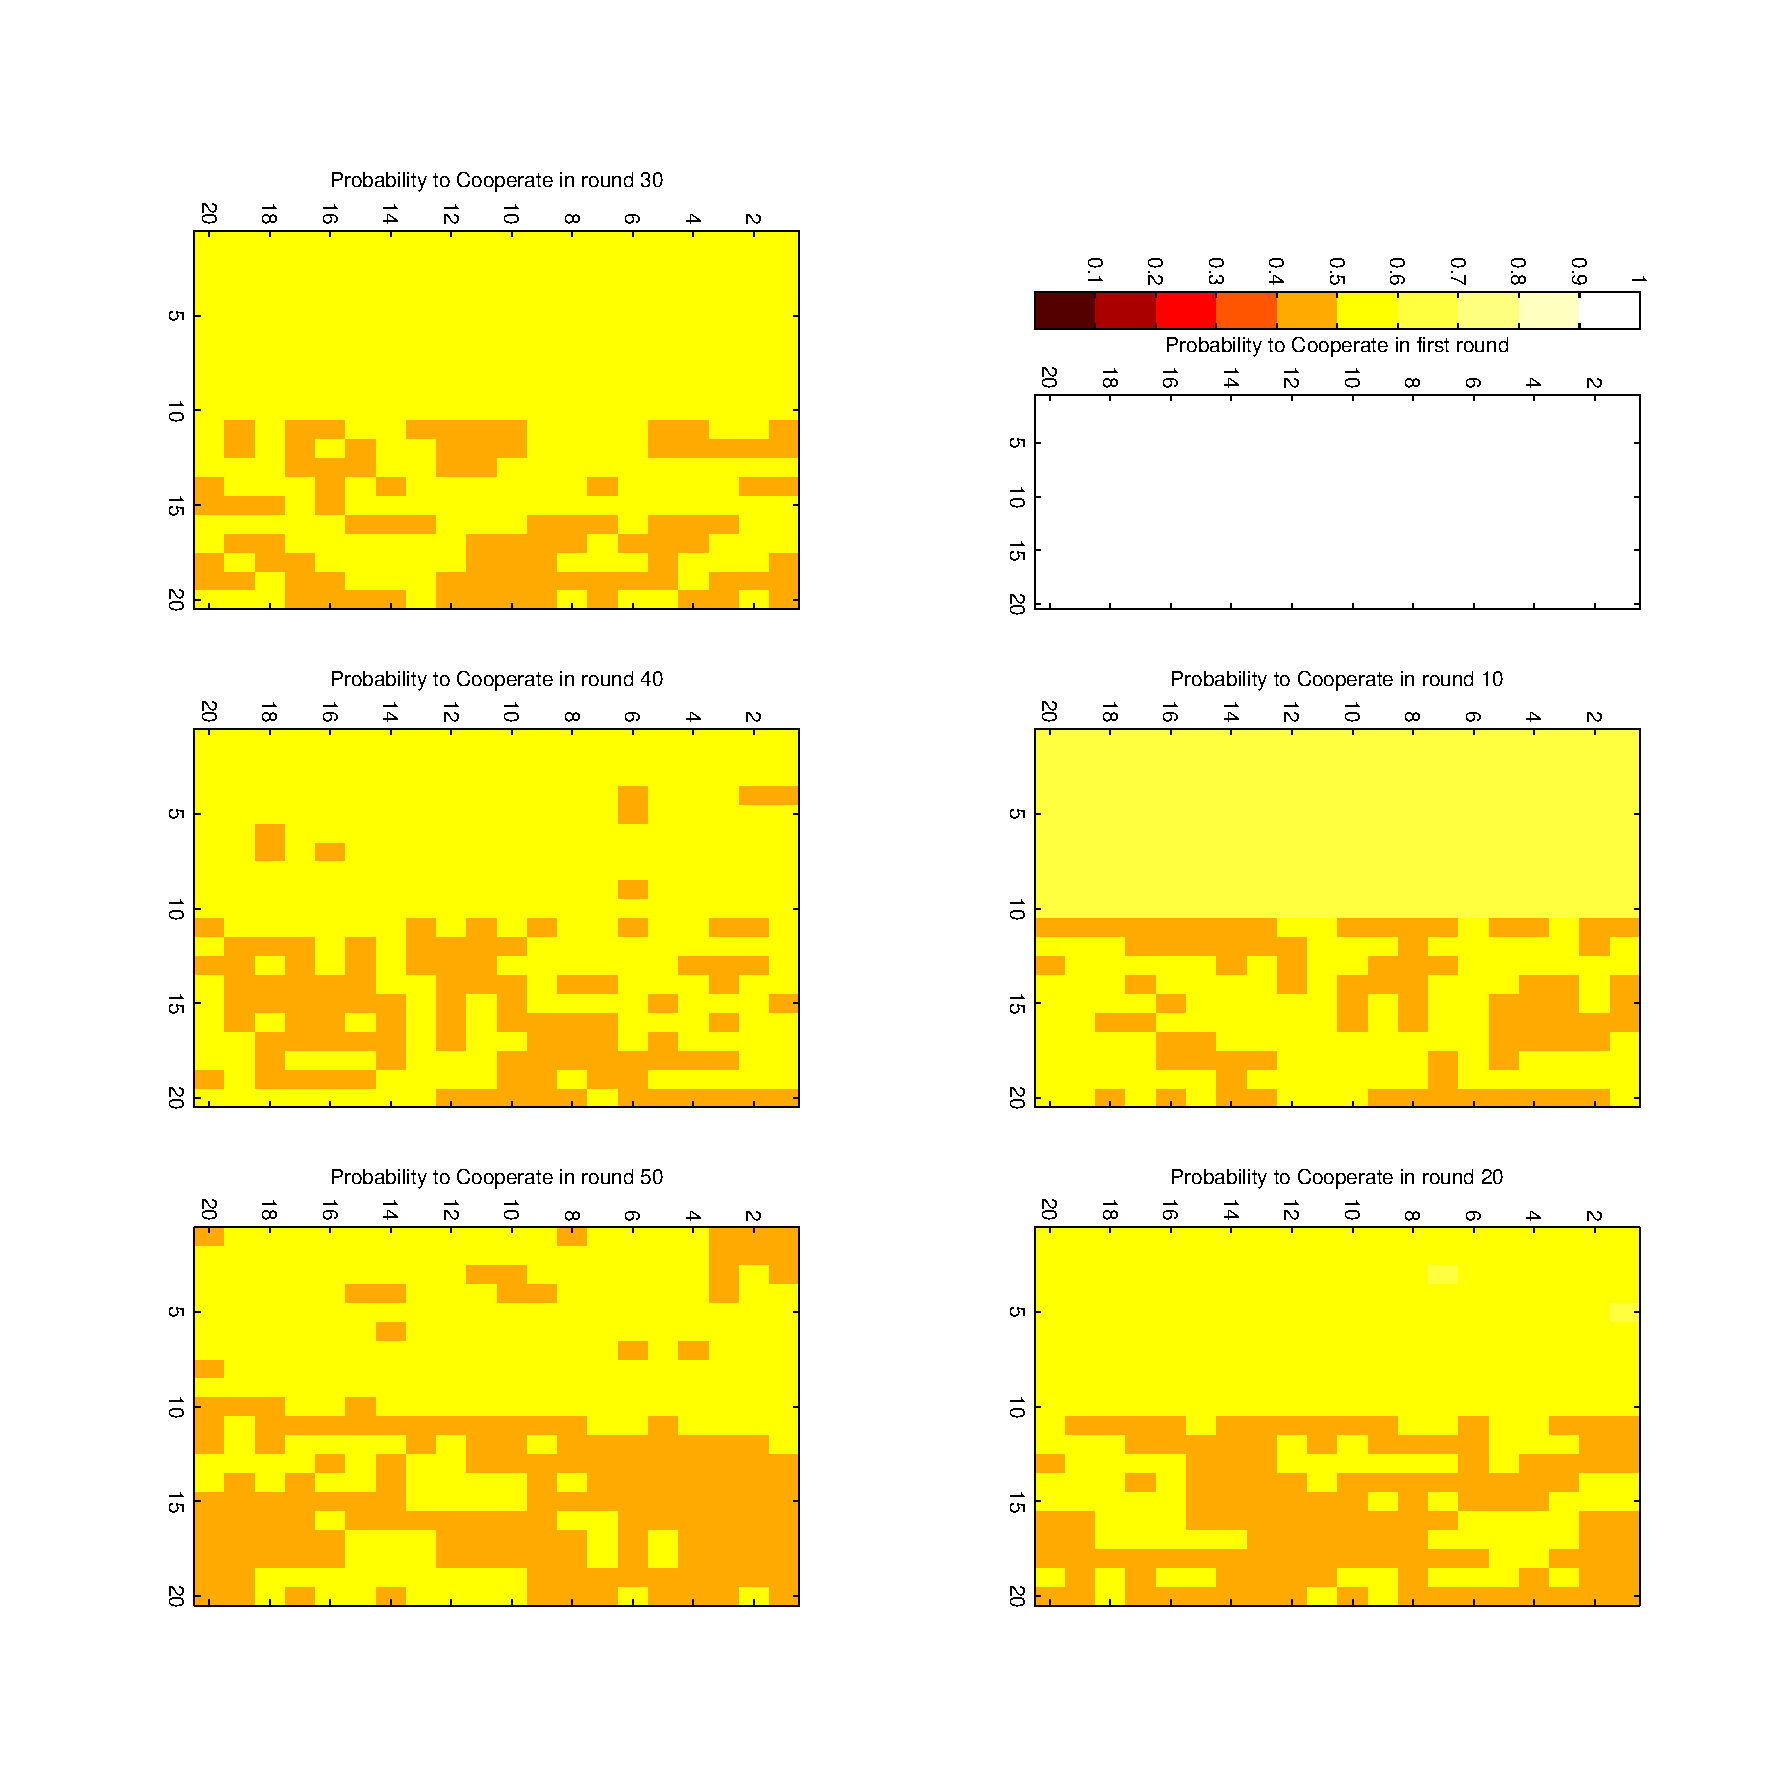
\includegraphics[scale=0.6]{ProbabilityToCooperateInDiffRound30.pdf}
\caption[]{This is the probability for cooperation each Player for 6 rounds ( 1 , 10, 20, 30, 40 and 60). One played over 50 rounds with 400 players and middled over 40 simulations. The initial conditions were set such that: the aspiration is for everybody 3, the initial probability for cooperation is1 for everyone. The strategy is distributed such that the upper half of the players have a lower learning rate (0.5) then the rest (0.8) }
\label{exp30}
\end{figure}

\begin{figure}
\centering
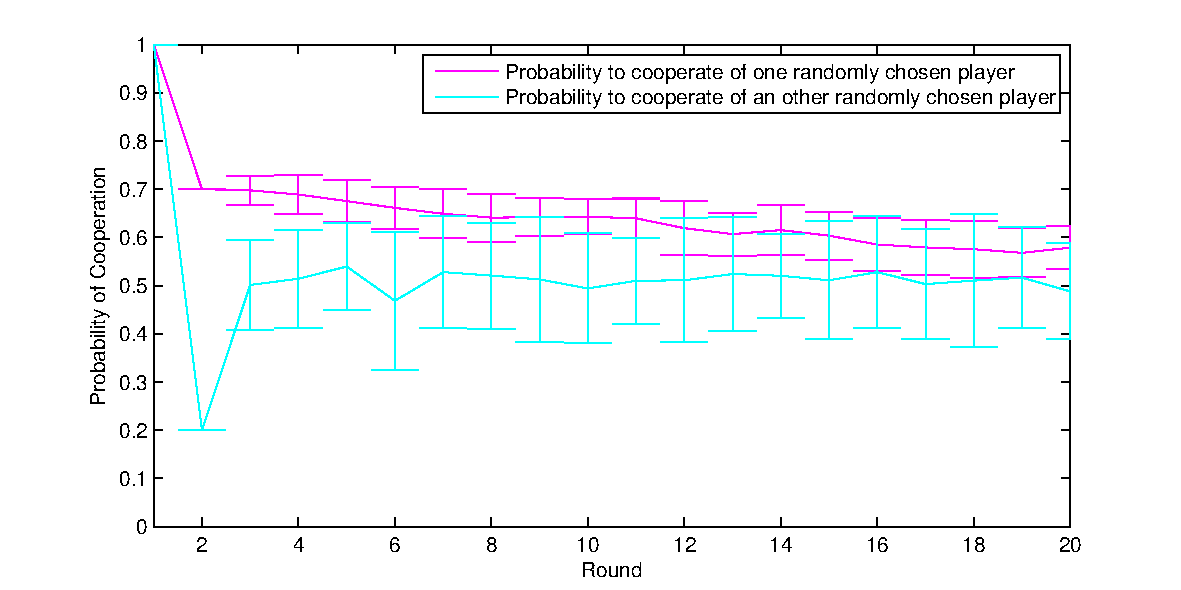
\includegraphics[scale=0.8]{ProbCoopwithtime30.pdf}
\caption[]{This is the probability for cooperation for 2 Players (one from the top and one from the bottom) plottet for each round. One played over 20 rounds with 400 players and middled over 40 simulations.  The initial conditions were set such that: the aspiration is for everybody 3, the initial probability for cooperation is1 for everyone. The strategy is distributed such that the upper half of the players have a lower learning rate (0.5) then the rest (0.8)}
\label{exp30time}
\end{figure}
In figure \ref{exp33} we want outpoint the final score of the players. The experiment is here defiend with the initial conditions: the aspiration is 3 for all players, the probability for cooperation is 1 for a defined quarter which has the strategy of only cooperation, where as the rest has the initial probability of cooperation of 0.5 and the strategy of learning with a learning rate of 0.8. 
\\One can see that the players in the defined quarter have a much higher score than the ones which cooperated all the time have a significant higher score than the ones which have made their decisions ased on learning. We also made this experiment with only a small neighbourhood instead of a whole quarter. There they profited even more of their situation.

\begin{figure}
\centering
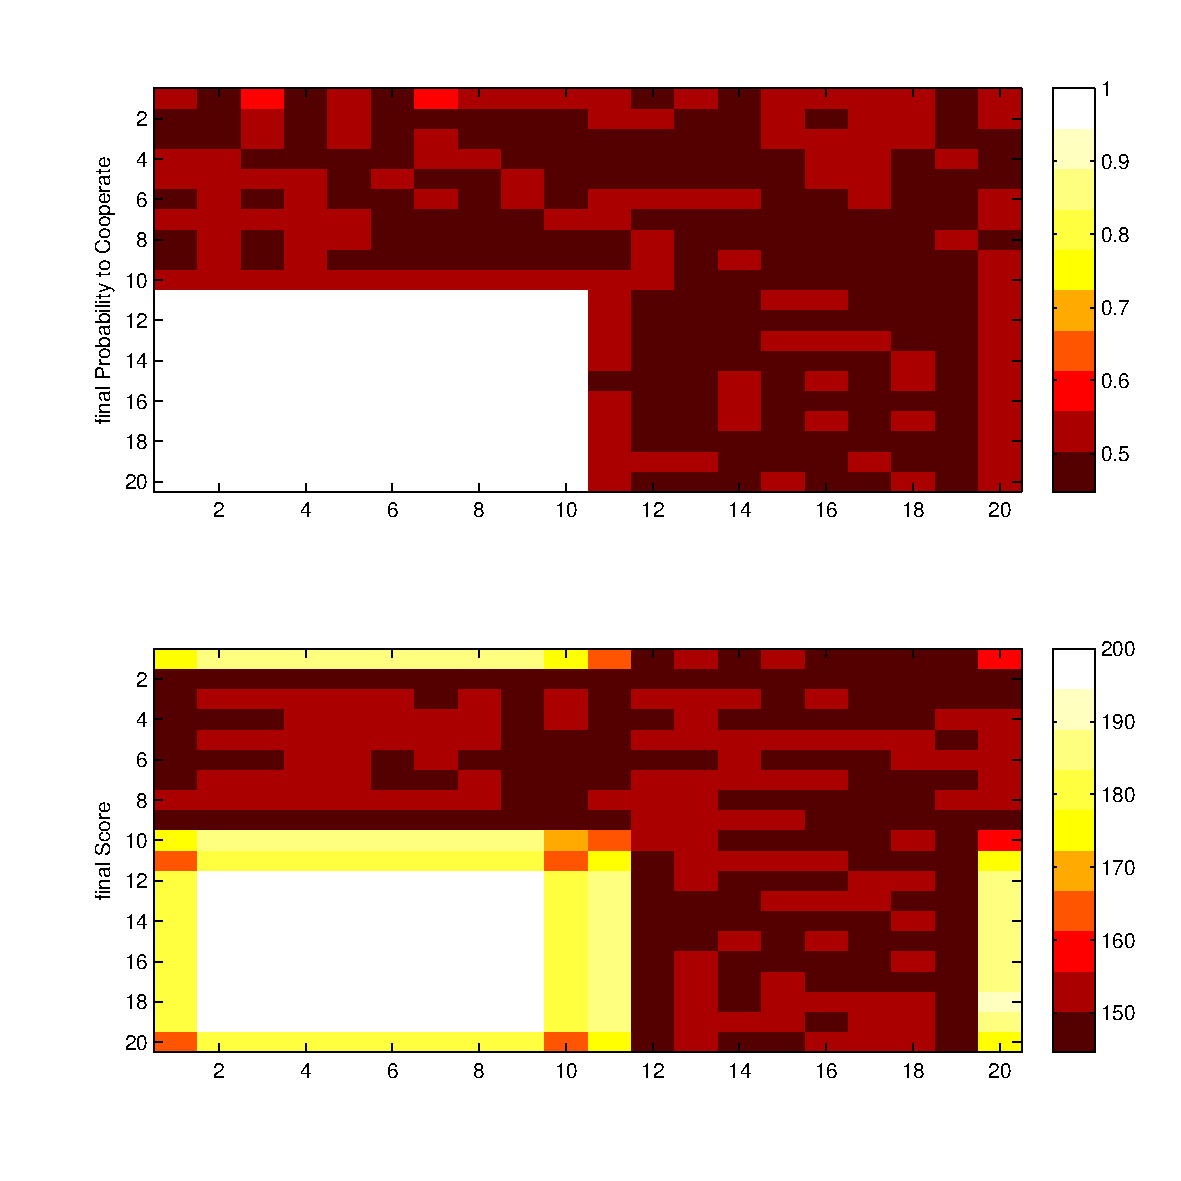
\includegraphics[scale=0.6]{ScoreAndProbcoopWithImagesc33.pdf}
\caption[]{This is the final probability for cooperation and the score of each Player. One played over 50 rounds with 400 players and middled over 40 simulations. The initial conditions were set such that: the aspiration is 3 for all players, the probability for cooperation is 1 for a defined quarter which has the strategy of only cooperation, where as the rest has the initial probability of cooperation of 0.5 and the strategy of learning with a learning rate of 0.8. }
\label{exp33}
\end{figure}
%%%%%%%%%%%%%%%%%%%%%%%%%%%%%%%%%%%%%%%%%%%%%%%%%%%%%%%%%%%%%%%%%%%%%%%%%%%


\section{Summary and Outlook}

The Replicator Dynamics are very useful for mathamatical analysis. There is a hunge potential in further Replicator Dynamics models including more players while considering more complicated effects of more complex games. As can be seen in this report, only a slight change of the model of the Chicken Dilemma may lead to non-linear highly complex systems. Even only be changing the constant parameters of the Chicken Dilemma may lead to different results. Obviously there is a high potential of adding additional configurations to the model. The high complexity of further models implies that there is still a huge potential in more research on this issue of a complex system.
Nevertheless, the Replicator Dynamics model is quiet different to those of the Cellular Automaton. The Replicator Dynamics assume perfect evolutinary behavior whereas the Cellular Automaton does not. Thus, the Replicator Dynamics only give useful results for theory but not for real game theory. The Replicator Dynamics show what is possible and what is not but they are not able to forecast random effects as random noise. 
\\From the bigger model of the implemented Chicken Dilemma one can learn, that there wont build sponaniously any cluster if one does not define any special initial conditions. Not even when one build in peer pressure with the modeled learning strategy. Also significant is that in almost all cases of initially varying conditions between the players, the dynamics smooves out and find it's stable state at a probability of cooperation around 0.5. The only case, where a non trivial distribution of cooperation probability remains is when one defines an initially sinusoidal distribution of probabilities.
\\One can also outpoint, that in respect to the final score it is better to sit in a pool of cooperators when the rest takes decision based on other strategies then sitting outside.
\\If one has one population which has the strategy of Learning and another which keep its initial probability of cooperation, the population of learners will only converge to the others if the others have a higher probability of cooperation.



\section{References}

\begin{enumerate}
\item Michael W. Macy, Andreas Flache ; \itshape {Learning Dynamics in social dilemmas};\upshape  1999
\item Daniel Friedman; \itshape {Evolutionary Games in Economics};\upshape  1991
\item Neugebauer, Poulsen, Schram; \itshape{Fairness and reciprocity in the Hawk-Dove Game};\upshape  2003
\end{enumerate}




\end{document}  



 
